\subsection{比较关系：I. 弱关系}

在下文中，我们用 V 表示赋值域 K 上的一个赋范向量空间，并用 \(\mathcal{H}(\mathfrak{F}, V)\) 表示取值于 V 且各自定义在 E 的属于滤子基 F 的某个子集上的函数所成的集。我们将要在这些函数之间定义的关系，相对于以 F 为基的滤子具有局部性：我们来明确这句话的含义。设 f 与 g 是 \(\mathcal{H}(\mathfrak{F}, V)\) 中的两个函数，回忆一下，关系“存在一个集 \(Z \in F\) ，使 f 与 g 在 Z 上都有定义且相等”是一个等价关系 \(R_{\infty}\) ，定义在 \(\mathcal{H}(\mathfrak{F}, V)\) 上 (Gen.~Top., I, p.~66)。在此情形下，若含 \(\mathcal{H}(\mathfrak{F}, V)\) 中一个函数 f 的关系 S（关于 f）与等价关系 \(R_{\infty}\) 相容 (Set Theory, II, p.~117)，我们就说它（沿 F）关于 f 具有局部性；我们知道，如果 \(\tilde{f}\) 是 f 沿 F 的芽，即 f 模 \(R_{\infty}\) 的等价类（商集 \(\mathcal{H}_{\infty}(\mathfrak{F}, V) = \mathcal{H}(\mathfrak{F}, V)/R_{\infty}\) 中的一个元素），那么由 S 过渡到商，可以导出一个 \(\tilde{f}\) 与 S 的其余变元之间的关系；反之，每个这种形式的关系也定义一个关于 f 具有局部性的关系。

例. 设 f 与 g 是 \(\mathcal{H}(\mathfrak{F},\mathbf{R})\) 中的两个函数，关系“存在一个 \(X \in F\) ，使 f 与 g 都在 X 上有定义，且 \(f(t) \leqslant g(t)\) 对每个 \(t \in X\) 成立”关于 f 与 g 具有局部性。我们把（对 f 与 g）过渡到商所得到的关系记作 \(\tilde{f} \leqslant \tilde{g}\) ；我们指出，若 \(\tilde{f} \leqslant \tilde{g}\) ，则存在一个函数 \(f_{1} \in \tilde{f}\) 与一个函数 \(g_{1} \in \tilde{g}\) ，都定义在整个 E 上，使得 \(f_{1}(t) \leqslant g_{1}(t)\) 对一切 \(t \in E\) 成立。

注. 1) 设 \(V_{i}\) ( \(1 \leqslant i \leqslant n\) ) 是 K 上的 n 个赋范向量空间，\(\varphi\) 是定义在 \(V_{1} \times V_{2} \times \cdots \times V_{n}\) 上、取值于 V 的函数；沿 \(R_{\infty}\) 过渡到商，函数 \(\varphi\) 便定义了一个从

\[
\mathcal {H} _ {\infty} (\mathfrak {F}, V _ {1}) \times \dots \times \mathcal {H} _ {\infty} (\mathfrak {F}, V _ {n})
\]

到 \(\mathcal{H}_{\infty}(\mathfrak{F}, V)\) 中的映射，通常记作 \(\varphi(\tilde{\mathbf{f}}_1, \ldots, \tilde{\mathbf{f}}_n)\) (Gen.~Top., I, p.~67)。例如，取 \(\varphi\) 为映射 \((\mathbf{x}, \mathbf{y}) \mapsto \mathbf{x} + \mathbf{y}\) 与 \(\mathbf{x} \mapsto \mathbf{x}\lambda\) ( \(\lambda \in \mathbf{K}\) )，便对任意两个芽 \(\tilde{\mathbf{f}}\) 、 \(\tilde{\mathbf{g}}\) （均属于 \(\mathcal{H}_{\infty}(\mathfrak{F}, V)\) ）定义了元素 \(\tilde{\mathbf{f}} + \tilde{\mathbf{g}}\) 与 \(\tilde{\mathbf{f}}\lambda\) ，并且立即可验证，合成法则 \((\tilde{\mathbf{f}}, \tilde{\mathbf{g}}) \mapsto \tilde{\mathbf{f}} + \tilde{\mathbf{g}}\) 与 \((\lambda, \tilde{\mathbf{f}}) \mapsto \tilde{\mathbf{f}}\lambda\) 在 \(\mathcal{H}_{\infty}(\mathfrak{F}, V)\) 上定义了域 \(\mathbf{K}\) 上的一个向量空间结构；在这个空间中，\(\tilde{0}\) 是由等于 \(0\) （于 \(\mathfrak{F}\) 的某个集上）的函数组成的类，而 \(-\tilde{\mathbf{f}}\) 是由等于 \(-\mathbf{f}\) （于 \(\mathfrak{F}\) 的某个集上）的函数组成的类。同样，若 \(V\) 是 \(K\) 上的一个代数，则对 \(\mathcal{H}_{\infty}(\mathfrak{F}, V)\) 定义第二个内合成法则 \((\tilde{\mathbf{f}}, \tilde{\mathbf{g}}) \mapsto \tilde{\mathbf{f}}\tilde{\mathbf{g}}\) （取 \(\varphi(\mathbf{x}, \mathbf{y}) = \mathbf{x}\mathbf{y}\) ）；它与前两个法则一起，定义了 \(K\) 上的一个代数结构于 \(\mathcal{H}_{\infty}(\mathfrak{F}, V)\) 上；若 \(V\) 具有单位元 \(\mathbf{e}\) ，则 \(\mathcal{H}_{\infty}(\mathfrak{F}, V)\) 以类 \(\tilde{\mathbf{e}}\) 为单位元，该类由等于 \(\mathbf{e}\) 于 \(\mathfrak{F}\) 的某个集上的函数组成；为使 \(\tilde{\mathbf{f}}\) 在 \(\mathcal{H}_{\infty}(\mathfrak{F}, V)\) 中可逆，必须且只需：对某个 \(\mathbf{f} \in \tilde{\mathbf{f}}\) ，存在一个 \(Z \in \mathfrak{F}\) ，使得 \(\mathbf{f}(t)\) 在 \(V\) 中对每个 \(t \in Z\) 都可逆（这时，类 \(\tilde{\mathbf{f}}\) 中每个函数都满足这一条件）。

\begin{enumerate}
\def\labelenumi{\arabic{enumi})}
\setcounter{enumi}{1}
\tightlist
\item
  沿用同样的记号，设 \(\psi\) 是 \(\prod_{i=1}^{n} V_i\) 的一个子集到 \(V\) 中的映射；我们以 \(\psi(\mathbf{f}_1, \mathbf{f}_2, \ldots, \mathbf{f}_n)\) 表示这样的函数，它等于 \(\psi(\mathbf{f}_1(t), \mathbf{f}_2(t), \ldots, \mathbf{f}_n(t))\) 于每个点 \(t \in E\) （在该点诸 \(\mathbf{f}_i(t)\) 有定义，且点 \((\mathbf{f}_i(t))\) 属于 \(\psi\) 的定义集）\(^1\) 。例如，\(\mathbf{f} + \mathbf{g}\) 就是等于 \(\mathbf{f}(t) + \mathbf{g}(t)\) 于每个点 \(t \in E\) （\(\mathbf{f}\) 与 \(\mathbf{g}\) 在该点都有定义）的函数。注意，映射 \((\mathbf{f}, \mathbf{g}) \mapsto \mathbf{f} + \mathbf{g}\) 不是 \(\mathcal{H}(\mathfrak{F}, V)\) 上的一个群律，因为若 \(\mathbf{f}\) 不在整个 \(E\) 上有定义，则不存在函数 \(\mathbf{g} \in \mathcal{H}(\mathfrak{F}, V)\) 使 \(\mathbf{f} + \mathbf{g} = 0\) 。
\end{enumerate}

定义 1. 给定两个实函数 \(f, g\) ，它们属于 \(\mathcal{H}(\mathfrak{F}, \mathbf{R})\) 且 \(\geqslant 0\) 于 \(\mathfrak{F}\) 的某个集上，我们说 \(f\) 受 \(g\) 控制，或者说 \(g\) 控制 \(f\) （沿 \(\mathfrak{F}\) ），并记作 \(f \preccurlyeq g\) 或 \(g \succcurlyeq f\) ，如果存在一个集 \(X \in \mathfrak{F}\) 和一个数 \(k > 0\) ，使得 \(f(t) \leqslant k g(t)\) 对每个 \(t \in X\) 成立（换句话说，如果存在 \(k > 0\) 使 \(\tilde{f} \leqslant k \tilde{g}\) ）

给定两个赋范向量空间 \(V_{1}, V_{2}\) ，以及两个函数 \(f_{1}, f_{2}\) ，分别属于 \(\mathcal{H}(\mathfrak{F}, V_{1})\) 与 \(\mathcal{H}(\mathfrak{F}, V_{2})\) ，我们说 \(f_{1}\) 受 \(f_{2}\) 控制（沿 \(F\) ），并记作 \(f_{1} \preccurlyeq f_{2}\) 或 \(f_{2} \succcurlyeq f_{1}\) ，如果 \(\|f_{1}\| \preccurlyeq \|f_{2}\|\) 。

关系 \(f_{1} \preccurlyeq f_{2}\) 显然关于 \(f_{1}\) 与 \(f_{2}\) 具有局部性；因此它等价于过渡到商所得到的关系 \(\tilde{f}_{1} \preccurlyeq \tilde{f}_{2}\) 。当 f 与 g 是实函数时，应当注意不要混淆关系 \(\tilde{f} \preccurlyeq \tilde{g}\) 与 \(\tilde{f} \leqslant \tilde{g}\) 。

注意，对每个标量 \(\lambda \neq 0\) ，关系 \(\mathbf{f}_1 \preccurlyeq \mathbf{f}_2\lambda\) 等价于 \(\mathbf{f}_1 \preccurlyeq \mathbf{f}_2\) 。若 \(\mathbf{f}_1 \preccurlyeq \mathbf{f}_2\) ，则存在一个集 \(X \in \mathfrak{F}\) ，使得 \(\mathbf{f}_1(x) = 0\) 对每个点 \(x \in X\) （在该点 \(\mathbf{f}_2(x) = 0\) ）成立。

例. 1) 关系 \(\mathbf{f} \preccurlyeq 1\) 表示 \(\mathbf{f}\) 在 \(\mathfrak{F}\) 的某个集上有界。

\begin{enumerate}
\def\labelenumi{\arabic{enumi})}
\setcounter{enumi}{1}
\item
  对每个函数 \(\mathbf{f}\) （属于 \(\mathcal{H}(\mathfrak{F}, V)\) ）以及每个标量 \(\lambda \neq 0\) ，有 \(\mathbf{f} \preccurlyeq \mathbf{f}\lambda\) 。
\item
  当 \(x\) 趋于 \(+\infty\) 时，有 \(\sin^2 x \preccurlyeq \sin x\) 。
\item
  当 \((x,y)\) 趋于 \((0,0)\) （在 \(\mathbf{R}^2\) 中）时，有
\end{enumerate}

\[
x y \preccurlyeq x ^ {2} + y ^ {2}.
\]

下列命题是定义 1 的直接推论：

命题 1. 若 \(f, g, h\) 是 \(\mathcal{H}(\mathfrak{F}, \mathbf{R})\) 中的三个函数，则关系 \(f \preccurlyeq g\) 与 \(g \preccurlyeq h\) 蕴含 \(f \preccurlyeq h\) 。

命题 2. 设 \(\mathbf{f}_1, \mathbf{f}_2\) 是 \(\mathcal{H}(\mathfrak{F}, V)\) 中的两个函数，\(g\) 是 \(\mathcal{H}(\mathfrak{F}, \mathbf{R})\) 中的一个函数。关系 \(\mathbf{f}_1 \preccurlyeq g\) 与 \(\mathbf{f}_2 \preccurlyeq g\) 蕴含 \(\mathbf{f}_1 + \mathbf{f}_2 \preccurlyeq g\) 。

进一步：

命题 3. 设 \(V_{1}, V_{2}, V\) 是同一赋值域上的三个赋范空间，\((\mathbf{x}, \mathbf{y}) \mapsto [\mathbf{x}, \mathbf{y}]\) 是从 \(V_{1} \times V_{2}\) 到 V 中的一个双线性映射。若 \(f_{1}\) 与 \(f_{2}\) 分别是 \(\mathcal{H}(\mathfrak{F}, V_{1})\) 与 \(\mathcal{H}(\mathfrak{F}, V_{2})\) 中的函数，且 \(g_{1}, g_{2}\) 是 \(\mathcal{H}(\mathfrak{F}, \mathbf{R})\) 中使 \(f_{1} \preccurlyeq g_{1}\) 与 \(f_{2} \preccurlyeq g_{2}\) 成立的两个函数，则 \([f_{1}.f_{2}] \preccurlyeq g_{1}g_{2}\) 。

事实上，(Gen.~Top., IX, p.~173, th. 1) 存在一个数 \(a > 0\) ，使得 \(\|[\mathbf{f}_1.\mathbf{f}_2]\| \leqslant a\|\mathbf{f}_1\|\|\mathbf{f}_2\|\) 。

推论. 若 V 是一个赋范代数，\(f_{1}, f_{2}\) 是 \(\mathcal{H}(\mathfrak{F}, V)\) 中的两个函数，且 \(g_{1}, g_{2}\) 是 \(\mathcal{H}(\mathfrak{F}, \mathbf{R})\) 中的两个函数，则关系 \(f_{1} \preccurlyeq g_{1}\) 、 \(f_{2} \preccurlyeq g_{2}\) 蕴含 \(f_{1}f_{2} \preccurlyeq g_{1}g_{2}\) 。

由命题 1，关系 \(f \preccurlyeq g\) （\(\mathcal{H}(\mathfrak{F}, V)\) 中函数之间的）是传递的；又因它是自反的，关系“f \(\preccurlyeq g\) 且 \(g \preccurlyeq f\) ”是 \(\mathcal{H}(\mathfrak{F}, V)\) 上的一个等价关系 (Set Theory, II, p.~113)。

定义 2. 给定两个函数 \(\mathbf{f}\) 、 \(\mathbf{g}\) （属于 \(\mathcal{H}(\mathfrak{F}, V)\) ），我们说 \(\mathbf{f}\) 与 \(\mathbf{g}\) 相似（沿 \(\mathfrak{F}\) ），并记作 \(\mathbf{f} \asymp \mathbf{g}\) ，如果 \(\mathbf{f} \preccurlyeq \mathbf{g}\) 且 \(\mathbf{g} \preccurlyeq \mathbf{f}\) 。

对每个标量 \(\lambda \neq 0\) ，关系 \(\mathbf{f} \asymp \mathbf{g}\) 等价于 \(\mathbf{f} \asymp \mathbf{g}\lambda\) 。它蕴含存在一个集 \(X \in \mathfrak{F}\) ，使得 \(X\) 中使 \(\mathbf{f}(x) = 0\) 的点所成的子集与 \(X\) 中使 \(\mathbf{g}(x) = 0\) 的点所成的子集相同。

例. 1) 对实函数 \(f \in \mathcal{H}(\mathfrak{F}, \mathbf{R})\) 而言，关系 \(f \asymp 1\) 表示存在两个数 \(a > 0\) 、 \(b > 0\) ，使得 \(a \leqslant |f(x)| \leqslant b\) 于 \(\mathfrak{F}\) 的某个集上成立，或者表示函数 \(\log |f|\) 在 \(\mathfrak{F}\) 的某个集上有界：这时称 \(f\) 在 \(\mathfrak{F}\) 的某个集上对数有界。

\begin{enumerate}
\def\labelenumi{\arabic{enumi})}
\setcounter{enumi}{1}
\item
  设 V 是非离散赋值域 K 上的一个赋范空间，\(\mathbf{f}(x)=\mathbf{a}_{0}x^{n}+\mathbf{a}_{1}x^{n-1}+\cdots+\mathbf{a}_{n}\) 是变元 \(x\in K\) 的、以 V 为系数集的多项式，且 \(a_{0}\neq0\) 。对每个向量 \(b\neq0\) ，有 \(\mathbf{f}(x)\asymp\mathbf{b}x^{n}\) （当 \(|x|\) 趋于 \(+\infty\) ）。
\item
  我们已经看到 \(\sin^2 x \preccurlyeq \sin x\) （当 \(x\) 趋于 \(+\infty\) 时），但 \(\sin^2 x \asymp \sin x\) 并不成立，尽管这两个函数在相同的点处为零。
\item
  有 \(x^{2} + xy + y^{2} \asymp x^{2} + y^{2}\) （当 \((x, y)\) 趋于 \((0, 0)\) ，在 \(\mathbf{R}^2\) 中），但 \(xy \asymp x^{2} + y^{2}\) 不成立。
\end{enumerate}

由 V, p.~213 的命题 3 立即得出：若 \(f_1\) 、 \(f_2\) 、 \(g_1\) 、 \(g_2\) 是 \(\mathcal{H}(\mathfrak{F},\mathrm{K})\) 中的函数（K 为任一赋值域），则关系 \(f_1 \asymp g_1\) 与 \(f_2 \asymp g_2\) 蕴含 \(f_1f_2 \asymp g_1g_2\) 。

我们指出，与此相反，关系 \(f_{1} \asymp g_{1}\) 与 \(f_{2} \asymp g_{2}\) 并不蕴含 \(f_{1} + f_{2} \asymp g_{1} + g_{2}\) ，例如 \(f_{1}(x) = g_{1}(x) = x^{2}\) 、 \(f_{2}(x) = -(x^{2} + x)\) 、 \(g_{2}(x) = -(x^{2} - 1)\) （当实变量 \(x\) 趋于 \(+\infty\) ）便说明了这一点。

比较关系 \(f \preccurlyeq g\) 、 \(f \asymp g\) 称为弱关系。我们说 \(\mathcal{H}(\mathfrak{F}, V)\) 中的两个函数 f 、 g 是弱可比较的，如果它们满足关系 \(f \preccurlyeq g\) 、 \(g \preccurlyeq f\) 中的至少一个。

注. 1) \(\mathcal{H}(\mathfrak{F},\mathbf{R})\) 中的两个函数未必弱可比较，例如函数 1 与 \(x\sin x\) （当 \(x\) 趋于 \(+\infty\) ）便说明了这一点。

\begin{enumerate}
\def\labelenumi{\arabic{enumi})}
\setcounter{enumi}{1}
\tightlist
\item
  用 \(\mathbf{R}_0\) 表示关系 \(\mathbf{f} \asymp \mathbf{g}\) （在 \(\mathcal{H}(\mathfrak{F}, V)\) 上），用 \(\mathcal{H}_0(\mathfrak{F}, V)\) 表示商集 \(\mathcal{H}(\mathfrak{F}, V)/\mathrm{R}_0\) ；注意关系 \(\mathrm{R}_{\infty}\) 蕴含 \(\mathbf{R}_0\) 。对关系 \(\mathbf{f} \preccurlyeq \mathbf{g}\) 过渡到商，由 V, p.~213 的命题 1 便得到 \(\mathcal{H}_0(\mathfrak{F}, V)\) 上的一个序关系 (Set Theory, III, p.~134)；前一例子表明 \(\mathcal{H}_0(\mathfrak{F}, V)\) 并不被这个关系全序化。
\end{enumerate}

\subsection{比较关系：II. 强关系}

定义 3. 给定两个实函数 \(f, g\) ，它们属于 \(\mathcal{H}(\mathfrak{F}, \mathbf{R})\) 且 \(\geqslant 0\) 于 \(\mathfrak{F}\) 的某个集上，我们说 \(f\) 相对于 \(g\) 可忽略，或者说 \(g\) 占优于 \(f\) （沿 \(\mathfrak{F}\) ），并记作 \(f \ll g\) 或 \(g \gg f\) ，如果对每个 \(\varepsilon > 0\) ，存在一个集 \(X \in \mathfrak{F}\) ，使得 \(f(t) \leqslant \varepsilon g(t)\) 对每个 \(t \in X\) 成立。

给定两个赋范空间 \(V_{1}\) 、 \(V_{2}\) 以及两个函数 \(f_{1}\) 、 \(f_{2}\) ，它们分别属于 \(\mathcal{H}(\mathfrak{F}, V_{1})\) 与 \(\mathcal{H}(\mathfrak{F}, V_{2})\) ，我们说 \(f_{1}\) 相对于 \(f_{2}\) 可忽略（沿 \(F\) ），并记作 \(f_{1} \ll f_{2}\) 或 \(f_{2} \gg f_{1}\) ，如果 \(\|f_{1}\| \ll \|f_{2}\|\) 。

对每个标量 \(\lambda \neq 0\) ，关系 \(\mathbf{f}_1 \ll \mathbf{f}_2\lambda\) 等价于 \(\mathbf{f}_1 \ll \mathbf{f}_2\) 。关系 \(\mathbf{f}_1 \ll \mathbf{f}_2\) 蕴含 \(\mathbf{f}_1 \preccurlyeq \mathbf{f}_2\) ，但与之不等价。

注意，关系 \(f_{1} \preccurlyeq f_{2}\) 决不蕴含关系 “ \(f_{1} \ll f_{2}\) 或 \(f_{1} \asymp f_{2}\) ”：有 \(\sin x \preccurlyeq 1\) （当 x 趋于 \(+\infty\) 时），但关系 \(\sin x \ll 1\) 与 \(\sin x \asymp 1\) 中没有一个成立。

例. 1) 关系 \(\mathbf{f} \ll 1\) 表示 \(\mathbf{f}\) 沿 \(\mathfrak{F}\) 趋于 0。

\begin{enumerate}
\def\labelenumi{\arabic{enumi})}
\setcounter{enumi}{1}
\item
  当 \(\alpha\) 与 \(\beta\) 是两个实数且 \(\alpha < \beta\) 时，有 \(x^{\alpha} \ll x^{\beta}\) （当 \(x\) 趋于 \(+\infty\) 时）。类似地，当 \(m\) 与 \(n\) 是两个有理整数且 \(m < n\) 时，有 \(z^{m} \ll z^{n}\) （当复数 \(z\) 趋于 \(\infty\) 时）。
\item
  当 \(x\) 趋于 \(+\infty\) 时，有 \(x^n \ll e^x\) （对每个整数 \(n\) ）(III, p.~105)。
\item
  在 \(R^{2}\) 中，当 \((x, y)\) 趋于 \((0, 0)\) 时，有
\end{enumerate}

\[
x ^ {2} + y ^ {2} \ll | x | + | y |.
\]

下列命题可以由定义 3 立即推出：

命题 4. 若 \(f, g, h\) 是 \(\mathcal{H}(\mathfrak{F}, \mathbf{R})\) 中的三个函数，则关系 \(f \preccurlyeq g\) 与 \(g \ll h\) （相应地， \(f \ll g\) 与 \(g \preccurlyeq h\) ）蕴含 \(f \ll h\) 。

命题 5. 设 \(\mathbf{f}_1, \mathbf{f}_2\) 是 \(\mathcal{H}(\mathfrak{F}, V)\) 中的两个函数， \(g\) 是 \(\mathcal{H}(\mathfrak{F}, \mathbf{R})\) 中的一个函数。则关系 \(\mathbf{f}_1 \ll g\) 与 \(\mathbf{f}_2 \ll g\) 蕴含 \(\mathbf{f}_1 + \mathbf{f}_2 \ll g\) 。

此外，与 V, p.~213 的命题 3 中相同的论证表明：

命题 6. 采用命题 3 的记号，关系 \(\mathbf{f}_1 \ll g_1\) 与 \(\mathbf{f}_2 \preccurlyeq g_2\) （相应地， \(\mathbf{f}_1 \preccurlyeq g_1\) 与 \(\mathbf{f}_2 \ll g_2\) ）蕴含 \([\mathbf{f}_1.\mathbf{f}_2] \ll g_1g_2\) 。

命题 4 表明，关系 \(\mathbf{f} \ll \mathbf{g}\) （ \(\mathcal{H}(\mathfrak{F}, V)\) 中函数之间的）是传递的；但它不是自反的：确切地说，关系 \(\mathbf{f} \ll \mathbf{f}\) 蕴含 \(\mathbf{f}\) 在 \(\mathfrak{F}\) 的某个集上为零（换句话说， \(\mathbf{f}\) 模 \(R_{\infty}\) 等价于 0）；事实上，对一个 \(\varepsilon\) （满足 \(0 < \varepsilon < 1\) ），存在一个 \(X \in \mathfrak{F}\) ，使得 \(\| \mathbf{f}(x) \| \leqslant \varepsilon \| \mathbf{f}(x) \|\) 对每个 \(x \in X\) 成立，而这只有当 \(\mathbf{f}(x) = 0\) 对每个 \(x \in X\) 成立时才可能。由此推出，关系 “ \(\mathbf{f} \ll \mathbf{g}\) 且 \(\mathbf{g} \ll \mathbf{f}\) ” 是传递的和对称的，但不是自反的：因而它不是一个等价关系（它蕴含存在一个集 \(X \in \mathfrak{F}\) ，使得 \(\mathbf{f}(x) = \mathbf{g}(x) = 0\) 对每个 \(x \in X\) 成立）。

命题 7. 若 \(\mathbf{f}\) 与 \(\mathbf{g}\) 是 \(\mathcal{H}(\mathfrak{F}, V)\) 中的两个函数，则关系 \(\mathbf{f} - \mathbf{g} \ll \mathbf{f}\) 等价于 \(\mathbf{f} - \mathbf{g} \ll \mathbf{g}\) 。

事实上， \(\mathbf{f} - \mathbf{g} \ll \mathbf{f}\) 蕴含：对每个 \(\varepsilon > 0\) ，存在一个 \(X \in \mathfrak{F}\) ，使得 \(\| \mathbf{f}(x) - \mathbf{g}(x) \| \leqslant \varepsilon \| \mathbf{f}(x) \|\) 对每个 \(x \in X\) 成立。但这时 \((1 - \varepsilon) \| \mathbf{f}(x) \| \leqslant \| \mathbf{g}(x) \|\) ，从而 \(\mathbf{f} \preccurlyeq \mathbf{g}\) ，由此 (V, p.~215, prop. 4) 得 \(\mathbf{f} - \mathbf{g} \ll \mathbf{g}\) 。

推论. 关系 \(f - g \ll f\) 是 \(\mathcal{H}(\mathfrak{F}, V)\) 上的一个等价关系。

事实上，若 \(f - g \ll f\) 且 \(g - h \ll g\) ，则 \(f - g \ll g\) ，由此 (V, p.~215, prop. 5) 得 \(f - h \ll g\) ，于是，由于 \(g \preccurlyeq f\) ，我们有 \(f - h \ll f\) ，这表明该关系是传递的；它由命题 7 是对称的，且显然是自反的，由此得该推论。

定义 4. 给定 \(\mathcal{H}(\mathfrak{F}, V)\) 中的两个函数 f, g，我们说 f 与 g 等价（沿 F），并记作 \(f \sim g\) ，如果 \(f - g \ll f\) 。

关系 \(\mathbf{f} \sim \mathbf{g}\) 蕴含 \(\mathbf{f} \asymp \mathbf{g}\) ，但与之不等价。

例. 1) 若 \(\mathbf{a}\) 是一个常值函数， \(\neq 0\) 于 \(\mathbf{E}\) 上，则关系 \(\mathbf{f} \sim \mathbf{a}\) 表示 \(\mathbf{f}\) 趋于 \(\mathbf{a}\) （沿 \(\mathfrak{F}\) ）。

\begin{enumerate}
\def\labelenumi{\arabic{enumi})}
\setcounter{enumi}{1}
\item
  设 V 是非离散赋值域 K 上的一个赋范空间，并设 \(\mathbf{f}(x)=\mathbf{a}_{0}x^{n}+\mathbf{a}_{1}x^{n-1}+\cdots+\mathbf{a}_{n}\) 是变量 \(x\in K\) 的一个多项式，其系数在 V 中，且满足 \(a_{0}\neq0\) 。则 \(f(x)\sim a_{0}x^{n}\) （当 \(|x|\) 趋于 \(+\infty\) 时）。
\item
  当实数 \(x\) 趋于 \(+\infty\) 时，有 \(\left(1 + \frac{1}{x}\right)\sin x \sim \sin x\) 。
\item
  当复变量 \(z\) 趋于 0 时，有 \(e^z - 1 \sim z\) 。更一般地，若 \(V\) 是赋值域 \(K\) 上的一个赋范空间， \(\mathbf{f}\) 是定义在 \(x_0 \in K\) 的一个邻域上、取值于 \(V\) 、且具有导数 \(\mathbf{f}'(x_0) \neq 0\) 于点 \(x_0\) 处的函数，则当 \(x\) 趋于 \(x_0\) 时，有 \(\mathbf{f}(x) - \mathbf{f}(x_0) \sim \mathbf{f}'(x_0)(x - x_0)\) (I, p.~3, def. 1)。
\item
  当 \((x, y)\) 趋于 \((0, 0)\) （在 \(R^{2}\) 中）时，有
\end{enumerate}

\[
\sqrt {\sin^ {2} x + \sin^ {2} y} \sim \sqrt {x ^ {2} + y ^ {2}}.
\]

\begin{enumerate}
\def\labelenumi{\arabic{enumi})}
\setcounter{enumi}{5}
\item
  设 \(f(x, y)\) 是两个实变量 x, y 的、以实数为系数的多项式，无常数项。若当 x 保持 \textgreater0 而趋于 0 时，存在一个函数 \(\varphi(x)\) ，它在区间 \([0, a]\) 上连续，且满足 \(\varphi(0) = 0\) 与 \(f(x, \varphi(x)) = 0\) （对 \(0 \leqslant x \leqslant a\) ），则可以证明，存在一个有理数 r 与一个实数 \(\lambda \neq 0\) ，使得 \(\varphi(x) \sim \lambda x^{r}\) (V, p.~259, exerc. 3)。
\item
  对每个 \(x > 0\) ，用 \(\pi(x)\) 表示 \(\leqslant x\) 的素数的个数；已经证明， \(\pi(x) \sim x / \log x\) （当 \(x\) 趋于 \(+\infty\) 时）。
\end{enumerate}

\pandocbounded{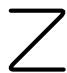
\includegraphics[keepaspectratio]{images/part002_abf04123.jpg}}

注. 注意，关系 \(\mathbf{f} \sim \mathbf{g}\) 决不蕴含差 \(\mathbf{f} - \mathbf{g}\) 沿 \(\mathfrak{F}\) 趋于 0；这个差甚至可以无界，正如例子 \(x^{2} + x \sim x^{2}\) （当 \(x\) 趋于 \(+\infty\) 时）所表明的。

命题 8. 设 K 是一个赋值域， \(f_{1}, f_{2}, g_{1}, g_{2}\) 是 \(\mathcal{H}(\mathfrak{F}, \mathrm{K})\) 中的四个函数；则关系 \(f_{1} \sim g_{1}\) 与 \(f_{2} \sim g_{2}\) 蕴含 \(f_{1}f_{2} \sim g_{1}g_{2}\) 。

事实上，我们有 \(f_{1}f_{2}-g_{1}g_{2}=f_{1}(f_{2}-g_{2})+(f_{1}-g_{1})g_{2}\) ；由于 \(f_{1}\preccurlyeq g_{1}\) 、 \(f_{1}-g_{1}\ll g_{1}\) 与 \(f_{2}-g_{2}\ll g_{2}\) ，我们有 \(f_{1}f_{2}-g_{1}g_{2}\ll g_{1}g_{2}\) (V, p.~215, prop. 5 and 6)。

相反，我们在 V, p.~214 中已给出一个例子，其中有 \(f_{1} = g_{1}\) 、 \(f_{2} \sim g_{2}\) ，然而关系 \(f_{1} + f_{2} \asymp g_{1} + g_{2}\) 并不成立（故更谈不上

\[
f _ {1} + f _ {2} \sim g _ {1} + g _ {2}).
\]

比较关系 \(f \ll g\) 、 \(f \sim g\) 称为强关系。 \(\mathcal{H}(\mathfrak{F}, V)\) 中的两个函数 f, g 称为可比较的（当想要避免任何可能的混淆时，称为强可比较的），如果它们满足下列三个关系之一： \(f \ll g\) 、 \(f \gg g\) ，或 “存在一个 \(\lambda \neq 0\) 使得 \(f \sim g\lambda\) ”。

注. 1) 两个函数可以是弱可比较的但不是强可比较的，例如函数 1 与 \(\sin x\) （当 \(x\) 趋于 \(+\infty\) 时）。

\begin{enumerate}
\def\labelenumi{\arabic{enumi})}
\setcounter{enumi}{1}
\tightlist
\item
  在比较关系 \(f_{1} \preccurlyeq f_{2}\) 与 \(f_{1} \ll f_{2}\) 的定义中，空间 \(V_{1}, V_{2}\) （ \(f_{1}\) 与 \(f_{2}\) 分别在其中取值）上的范数只是表面上介入；实际上介入的只是 \(V_{1}\) 与 \(V_{2}\) 上的拓扑，因为关系 \(f_{1} \preccurlyeq f_{2}\) 与 \(f_{1} \ll f_{2}\) 当把 \(V_{1}\) 或 \(V_{2}\) 上的范数换成一个等价范数时，就被等价的关系所代替 (Gen.~Top., IX, p.~170, def. 7)。
\end{enumerate}

\subsection{变量替换}

设 \(\varphi\) 是从集 \(E'\) 到 \(E\) 中的一个映射，使得 \(\overset{-1}{\varphi}(\mathfrak{F})\) 是 \(E'\) 上的一个滤子基。显然，若 \(\mathbf{f}_1, \mathbf{f}_2\) 分别是 \(\mathcal{H}(\mathfrak{F}, V_1)\) 与 \(\mathcal{H}(\mathfrak{F}, V_2)\) 中的函数，则 \(\mathbf{f}_1 \circ \varphi\) 、 \(\mathbf{f}_2 \circ \varphi\) 分别属于 \(\mathcal{H}(\overset{-1}{\varphi}(\mathfrak{F}), V_1)\) 与 \(\mathcal{H}(\overset{-1}{\varphi}(\mathfrak{F}), V_2)\) ，且关系 \(\mathbf{f}_1 \preccurlyeq \mathbf{f}_2\) （相应地， \(\mathbf{f}_1 \ll \mathbf{f}_2\) ）等价于 \(\mathbf{f}_1 \circ \varphi \preccurlyeq \mathbf{f}_2 \circ \varphi\) （相应地， \(\mathbf{f}_1 \circ \varphi \ll \mathbf{f}_2 \circ \varphi\) ）。

\subsection{严格正函数之间的比较关系}

设 \(g\) 是 \(\mathcal{H}(\mathfrak{F},\mathbf{R})\) 中的一个函数，它在 \(\mathfrak{F}\) 的某个集上严格正。涉及 \(g\) 的比较关系可以用另一种方式表述：关系 \(\mathbf{f} \preccurlyeq g\) 等价于说 \(\| \mathbf{f}\| /g\) （它定义在 \(\mathfrak{F}\) 的某个集上）在 \(\mathfrak{F}\) 的某个集上有界；关系 \(\mathbf{f} \ll g\) 等价于说 \(\| \mathbf{f}\| /g\) 沿 \(\mathfrak{F}\) 趋于 0。若 \(f\) 是 \(\mathcal{H}(\mathfrak{F},\mathbf{R})\) 中的一个函数，则关系 \(f\asymp g\) 表示 \(f / g\) 在 \(\mathfrak{F}\) 的某个集上对数有界，而关系 \(f\sim g\) 表示 \(f / g\) 沿 \(\mathfrak{F}\) 趋于 1。若 \(f\) 是 \(\mathcal{H}(\mathfrak{F},\mathbf{R})\) 中的一个函数且在 \(\mathfrak{F}\) 的某个集上为正，则说 \(f\) 与 \(g\) 可比较蕴含 \(f / g\) 趋于一个极限（有限的或等于 \(+\infty\) ，沿 \(\mathfrak{F}\) ）。

命题 9. 设 \(f\) 与 \(g\) 是 \(\mathcal{H}(\mathfrak{F},\mathbf{R})\) 中的两个函数，在 \(\mathfrak{F}\) 的某个集上严格正。为使 \(f\) 与 \(g\) 可比较，必要且充分的是：对每个数 \(t \geqslant 0\) （至多一个例外），函数 \(f - tg\) 具有常号 \(^3\) 于 \(\mathfrak{F}\) 的某个集上。

该条件是必要的。事实上，若 \(f \ll g\) ，则有 \(f - tg \sim -tg\) （ \(t = 0\) 除外），故 \(f - tg\) 在 \(\mathfrak{F}\) 的某个集上严格负（ \(t = 0\) 除外）；若 \(f \gg g\) ，则 \(f - tg\) 在 \(\mathfrak{F}\) 的某个集上严格正（对一切 \(t\) ）；最后，若 \(f \sim kg\) （ \(k\) 为常数 \(> 0\) ），则有 \(f - tg \sim (k - t)g\) （ \(t = k\) 除外），故除 \(t = k\) 可能例外外， \(f - tg\) 具有 \(k - t\) 的符号于 \(\mathfrak{F}\) 的某个集上。

该条件是充分的。事实上，设比值 \(f / g\) 有两个不同的聚点 \(\alpha < \beta\) （沿 \(\mathfrak{F}\) ）。于是对每个数 \(t\) （满足 \(\alpha < t < \beta\) ），在每个集 \(X \in \mathfrak{F}\) 中都存在两点 \(x_{1}, x_{2}\) ，使得 \(f(x_{1}) / g(x_{1}) < t\) 且 \(f(x_{2}) / g(x_{2}) > t\) ；从而 \(f(x) - tg(x)\) 在 \(X\) 上不具有常号；我们得到了一个与假设不相容的结论。由此推出， \(f / g\) 沿以 \(\mathfrak{F}\) 为基的滤子只能有一个聚值（有限的或无穷的），从而 (Gen.~Top., I, p.~85, corollary) 沿 \(\mathfrak{F}\) 以这个值为其极限。

命题 10. 设 \(f\) 与 \(g\) 是 \(\mathcal{H}(\mathfrak{F},\mathbf{R})\) 中的两个函数，在 \(\mathfrak{F}\) 的某个集上严格正；对每个实数 \(\alpha\) 且 \(\neq 0\) ，关系 \(f\asymp g\) （相应地， \(f\sim g\) ）等价于 \(f^{\alpha}\asymp g^{\alpha}\) （相应地， \(f^{\alpha}\sim g^{\alpha}\) ）；若 \(\alpha >0\) ，关系 \(f\preccurlyeq g\) （相应地， \(f\ll g\) ）等价于 \(f^{\alpha}\preccurlyeq g^{\alpha}\) （相应地， \(f^{\alpha}\ll g^{\alpha}\) ）；若 \(\alpha < 0\) ，它等价于 \(f^{\alpha}\succcurlyeq g^{\alpha}\) （相应地， \(f^{\alpha}\gg g^{\alpha}\) ）。

证明都是直接的。

我们注意到，在 \(\mathcal{H}(\mathfrak{F},\mathbf{R})\) 中，在 F 的某个集上严格正的函数所成的集 \(\varGamma\) 使得 \(\varGamma/\mathrm{R}_{\infty}\) 是一个乘法群 \(\varGamma_{\infty}\) （在 \(\mathcal{H}_{\infty}(\mathfrak{F},\mathbf{R})\) 中）； \(\varGamma/\mathrm{R}_{0}\) 恒同于 \(\varGamma_{\infty}\) 关于（模 \(R_{\infty}\) ） \(\varGamma\) 中对数有界函数的类所成的子群的商群；在 \(\varGamma/R_{0}\) 上，由关系 \(f \preccurlyeq g\) 通过过渡到商而导出的序关系与 \(\varGamma/R_{0}\) 的群结构相容，从而使之成为一个有序群。

命题 11. 设 g 是 \(\mathcal{H}(\mathfrak{F},\mathbf{R})\) 中的一个函数，使得 \(\lim_{\mathfrak{F}}g = +\infty\) ；则关系 \(f \ll g\) 蕴含 \(e^{f} \ll e^{g}\) ；关系 \(f \sim g\) 蕴含 \(\log f \sim \log g\) 。

事实上，若 \(f \ll g\) ，则 \(f - g = g\left(\frac{f}{g} - 1\right)\) 趋于 \(-\infty\) （沿 \(\mathfrak{F}\) ）。类似地，若 \(f \sim g\) ，则有 \(\log f = \log g + \log \frac{f}{g}\) ，故 \(\log f - \log g\) 趋于 0，对 \(\frac{\log f}{\log g} - 1 = \frac{\log f - \log g}{\log g}\) 亦然。

\pandocbounded{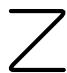
\includegraphics[keepaspectratio]{images/part002_2162bedd.jpg}}

另一方面，注意关系 \(f \sim g\) 并不蕴含 \(e^{f} \sim e^{g}\) ，甚至不蕴含 \(e^{f} \asymp e^{g}\) ，正如例子 \(f(x) = x^{2}\) 、 \(g(x) = x^{2} + x\) （当 x 趋于 \(+\infty\) 时）所表明的；类似地，关系 \(f \ll g\) 并不蕴含 \(\log f \ll \log g\) ，正如例子 \(f(x) = x\) 、 \(g(x) = x^{2}\) （当 x 趋于 \(+\infty\) 时）所表明的。

定义 5. 设 g 是 \(\mathcal{H}(\mathfrak{F},\mathbf{R})\) 中的一个函数，在 F 的某个集上严格正，且使得 \(\lim_{\mathfrak{F}}g=0\) 或 \(\lim_{\mathfrak{F}}g=+\infty\) 。我们说函数 \(f\in\mathcal{H}(\mathfrak{F},\mathbf{R})\) 相对于 g 是 \(\rho\) 阶的（有限或无穷），如果 \(\lim_{\mathfrak{F}}\log(|f|)/\log g=\rho\) 。

注意，若 f 相对于 g 是 \(\rho\) 阶的，则 f 相对于 1/g 是 \(-\rho\) 阶的；因此只需处理 \(g(x)\) 沿 F 趋于 \(+\infty\) 的情形。

\pandocbounded{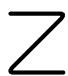
\includegraphics[keepaspectratio]{images/part002_5139c9a2.jpg}}

命题 12. 设 \(g\) 是 \(\mathcal{H}(\mathfrak{F},\mathbf{R})\) 中的一个函数，使得 \(\lim_{\mathfrak{F}}g = +\infty\) ；设 \(f\) 是 \(\mathcal{H}(\mathfrak{F},\mathbf{R})\) 中的一个函数。

\begin{enumerate}
\def\labelenumi{\alph{enumi})}
\item
  为使 \(f\) 是 \(+\infty\) 阶的（相对于 \(g\) ），必要且充分的是 \(f \gg g^{\alpha}\) （对每个 \(\alpha \geqslant 0\) ）。
\item
  为使 \(f\) 是 \(-\infty\) 阶的（相对于 \(g\) ），必要且充分的是 \(f \ll g^{-\alpha}\) （对每个 \(\alpha > 0\) ）。
\item
  为使 \(f\) 是等于 \(\rho\) 的有限阶（相对于 \(g\) ），必要且充分的是：对每个 \(\varepsilon > 0\) ，有 \(g^{\rho - \varepsilon} \ll f \ll g^{\rho + \varepsilon}\) 。
\end{enumerate}

例如我们证明 c)。若 \(f\) 相对于 \(g\) 的阶是 \(\rho\) ，则对每个 \(\varepsilon > 0\) ，存在一个集 \(\mathbf{M} \in \mathfrak{F}\) ，使得对每个 \(x \in \mathbf{M}\) ，我们有

\[
\left(\rho - \frac {\varepsilon}{2}\right) \log g (x) \leqslant \log | f (x) | \leqslant \left(\rho + \frac {\varepsilon}{2}\right) \log g (x),
\]

或者 \((g(x))^{\rho-\frac{\varepsilon}{2}} \leqslant |f(x)| \leqslant (g(x))^{\rho+\frac{\varepsilon}{2}}\) ；由于 \(\lim_{\mathfrak{F}} g = +\infty\) ，于是有 \(g^{\rho-\varepsilon} \ll f \ll g^{\rho+\varepsilon}\) （对每个 \(\varepsilon > 0\) ）；其逆是直接的。a) 与 b) 的证明类似。

注意，若 \(f\) 是有限阶 \(\rho\) （相对于 \(g\) ），则 \(fg^{-\rho}\) 相对于 \(g\) 是 0 阶，反之亦然；若 \(f_1\) （相应地， \(f_2\) ）是 \(\rho_1\) 阶（相应地， \(\rho_2\) 阶）的（相对于 \(g\) ），且 \(\rho_1 + \rho_2\) 有定义，则 \(f_1f_2\) 是 \(\rho_1 + \rho_2\) 阶的（相对于 \(g\) ）。

注. 1) 注意，尽管 f 相对于 g 可以是有限阶 \(\rho\) ，但比值 \(f/g^{\rho}\) 未必趋于一个极限；例如，每个对数有界函数相对于 g 都是 0 阶的，但沿 F 未必有极限。

\begin{enumerate}
\def\labelenumi{\arabic{enumi})}
\setcounter{enumi}{1}
\tightlist
\item
  一个定义在 \(\mathfrak{F}\) 的某个集上的函数未必相对于 \(g\) 有确定的阶（有限的或否），因为相对于 \(g\) 有确定阶的函数与 \(g\) 的一切幂可比较（至多一个例外）。而 \(f\) 未必具有这个性质，例子 \(g(x) = x\) 、 \(f(x) = 1 + x^2 \sin^2 x\) （当 \(x\) 趋于 \(+\infty\) 时）便表明了这一点。在这个例子中， \(f\) 与 \(g^\alpha\) 可比较（对 \(\alpha < 0\) 与 \(\alpha > 2\) ）；若取 \(f(x) = e^x \sin^2 x + e^{-x} \cos^2 x\) ，则 \(f\) 不与 \(g\) 的任何幂（正的或负的）可比较。
\end{enumerate}

\subsection{记号}

给定一个实函数 \(f \in \mathcal{H}(\mathfrak{F}, \mathbf{R})\) ，在一个公式中用 \(O(f)\) 表示一个受 \(f\) 控制的函数、用 \(o(f)\) 表示一个相对于 \(f\) 可忽略的函数，这往往是方便的。当在一个证明中出现多个受同一个函数 \(f\) 控制的（相应地，相对于 \(f\) 可忽略的）函数时，我们把它们记作 \(O_1(f)\) 、 \(O_2(f)\) 等（相应地， \(o_1(f)\) 、 \(o_2(f)\) 等）。

许多作者不加区分地把一个证明中所有受 f 控制的（相应地，相对于 f 可忽略的）函数都记作 \(O(f)\) （相应地， \(o(f)\) ），这是一种可能引起混淆的语言滥用。

用这个记号，我们可以把命题 1、2、3 (V, p.~213) 表述如下：若 \(g = O_1(f)\) 且 \(h = O(g)\) ，则 \(h = O_2(f)\) ；我们可以写

\[
\sum_ {i = 1} ^ {n} \lambda_ {i} O _ {i} (f) = O _ {n + 1} (f) \quad (\lambda_ {i} \text {   scalars })\tag{1}
\]

\[
O (f) O (g) = O (f g).\tag{2}
\]

类似地，命题 4 (V, p.~215) 表明，若 \(g = O_1(f)\) 且 \(h = o(g)\) （相应地， \(g = o_1(f)\) 且 \(h = O(g)\) ），则 \(h = o_2(f)\) ，而命题 5 与 6 (V, p.~5) 可以表述成形式

\[
\sum_ {i = 1} ^ {n} \lambda_ {i} o _ {i} (f) = o _ {n + 1} (f) \quad (\lambda_ {i} \text {   scalars })\tag{3}
\]

\[
o (f) O (g) = o (f g).\tag{4}
\]

关系 \(f \sim g\) 等价于 \(f = g + o(g)\) 。记号 \(O(1)\) （相应地， \(o(1)\) ）表示在 \(\mathfrak{F}\) 的某个集上有界的一个函数（相应地，沿 \(\mathfrak{F}\) 趋于 0 的一个函数）。

\section{渐近展开}

\subsection{比较尺度}

设 E 是一个被具有基 F 的滤子所滤过的集，K 是一个非离散赋值域（最常见的是 K = R 或 K = C）。在 \(\mathcal{H}(\mathfrak{F}, \mathrm{K})\) 中模 \(R_{\infty}\) 不等价于 0 的函数（即在 F 的每个集中至少有一点使函数不为零的那些函数）所成的集中，关系 “ \(f \ll g\) 或 f = g” 是一个序关系。

定义 1. 我们说 \(\mathcal{H}(\mathfrak{F},\mathrm{K})\) 的一个由模 \(R_{\infty}\) 不等价于 0 的函数组成的子集 E 是一个比较尺度，如果 E 被关系 “ \(f \ll g\) 或 f = g” 全序化。

换句话说，若 \(f\) 与 \(g\) 是 \(\mathcal{E}\) 中的函数，则关系 \(f \ll g\) 、 \(g \ll f\) 、 \(f = g\) 中总有一个（且只有一个）成立。由此推出，在 \(\mathcal{E}\) 上关系 \(f \asymp g\) （更不用说 \(|f| \sim a |g|\) ，其中 \(a\) 是一个数 \(> 0\) ）蕴含 \(f = g\) 。

一个比较尺度的每个子集显然也是一个比较尺度。

例. 1) 对实的且趋于 \(+\infty\) 的 x，函数 \(x^{\alpha}\) （ \(\alpha\) 为任意实数）所成的集是一个比较尺度。当 F 是以 a 为左端点的开区间所成的集时，函数 \((x - a)^{\alpha}\) 亦然。

\begin{enumerate}
\def\labelenumi{\arabic{enumi})}
\setcounter{enumi}{1}
\item
  当复数 \(z\) 趋于 \(\infty\) 时，函数 \(z^n\) （ \(n\) 为有理整数）所成的集是一个比较尺度；函数 \((z - a)^n\) 亦然（当 \(\mathfrak{F}\) 是该点的邻域滤子在点 \(a \in \mathbf{C}\) 的余集上的迹时）。
\item
  设 F 是赋范空间；当 F 是该点的邻域滤子在 a 的余集上的迹时，函数族 \(\|\mathbf{x}-\mathbf{a}\|^{\alpha}\) （ \(\alpha\) 为任意实数）是一个比较尺度。注意，若 p 与 q 是 F 上两个不同的范数，则两个比较尺度 \(\left(p(\mathbf{x}-\mathbf{a})\right)^{\alpha}\) 与 \(\left(q(\mathbf{x}-\mathbf{a})\right)^{\alpha}\) 的并一般不是一个比较尺度。
\item
  当实数 \(x\) 趋于 \(+\infty\) 时，函数族 \(\mathcal{E}\) 由形如 \(\exp(p(x))\) 的函数（其中 \(p\) 取遍无常数项的（实系数）多项式所成的集）组成，它是一个比较尺度：只需注意， \(\mathcal{E}\) 中两个函数的商仍在 \(\mathcal{E}\) 中，且函数 \(\exp(p(x))\) 必趋于 0 或 \(+\infty\) （如果 \(p \neq 0\) ）；事实上， \(p(x) \sim \alpha x^n\) （其中 \(n > 0\) 且 \(\alpha \neq 0\) ）；若 \(\alpha > 0\) ，则有 \(p(x) > \frac{1}{2}\alpha x^n\) （对充分大的 \(x\) ）；若 \(\alpha < 0\) ，则有 \(p(x) < \frac{1}{2}\alpha x^n\) （对充分大的 \(x\) ）；在第一种情形 \(\exp(p(x))\) 趋于 \(+\infty\) ，在第二种情形趋于 0。
\item
  对实的且趋于 \(+\infty\) 的 x，形如 \(x^{\alpha}(\log x)^{\beta}\) （对 x \textgreater{} 1 有定义）的函数所成的集 E（其中 \(\alpha\) 与 \(\beta\) 为任意实数）是一个比较尺度。事实上，这里同样，E 中两个函数的商是 E 中的一个函数；只需证明：若 \(\alpha\) 与 \(\beta\) 不全为零，则 \(x^{\alpha}(\log x)^{\beta}\) 趋于 0 或 \(+\infty\) ；这在 \(\alpha = 0, \beta \neq 0\) 时是明显的；若 \(\alpha > 0\) ，有 \((\log x)^{-\beta} \ll x^{\alpha}\) ，而若 \(\alpha < 0\) ，有 \((\log x)^{\beta} \ll x^{-\alpha}\) （对任何 \(\beta\) ），由此得命题。
\end{enumerate}

注意，最后这个比较尺度是一个全序集（对关系 “ \(f \ll g\) 或 \(f = g\) ”），其序结构同构于 \(R^{2}\) 上的字典序 (Set Theory, III, p.~157)；回忆在这个结构中关系 \((\alpha, \beta) < (\gamma, \delta)\) 表示 “ \(\alpha < \gamma\) ，或 \(\alpha = \gamma\) 且 \(\beta < \delta\) ”。

类似地，由函数 \(\exp(p(x))\) （其中 p 取遍无常数项多项式所成的集 \(P_{0}\) ）组成的尺度具有同构于 \(P_{0}\) 的序结构的序结构，在其中关系 p \textless{} q 表示多项式 q - p 的主导项具有 \textgreater{} 0 的系数 (cf.~Alg., VI. 19, 例 2)。

设 \(\varphi\) 是从集 \(F\) 到 \(E\) 中的一个映射，使得 \(\overset{-1}{\varphi}(\mathfrak{F})\) 是 \(F\) 上的一个滤子基。若 \(\mathcal{E}\) 是 \(E\) 上的一个比较尺度（对滤子基 \(\mathfrak{F}\) ），则函数 \(f \circ \varphi\) （当 \(f\) 取遍 \(\mathcal{E}\) ）在 \(F\) 上组成一个比较尺度（对滤子基 \(\overset{-1}{\varphi}(\mathfrak{F})\) ）。

\subsection{主部与渐近展开}

设 E 是一个由取值于非离散赋值域 K 中的函数组成的比较尺度。设 V 是 K 上的一个赋范空间，f 是 \(\mathcal{H}(\mathfrak{F}, V)\) 中的一个函数；如果存在一个函数 \(g \in E\) 和 V 中的一个元素 \(a \neq 0\) 使得 \(f \sim ag\) ，就说 ag 是 f 相对于尺度 E 的一个主部。由 V, p.~10 的定义 1，f 相对于 E 只能有一个主部，因为若 \(g_{1}\) 、 \(g_{2}\) 是 E 中的两个函数且 \(a_{1}\) 、 \(a_{2}\) 是 V 中两个 \(\neq 0\) 的元素，则关系 \(a_{1}g_{1} \sim a_{2}g_{2}\) 蕴含 \(|g_{1}| \asymp |g_{2}|\) ，从而 \(g_{1} = g_{2}\) ，于是 \((\mathbf{a}_{2} - \mathbf{a}_{1})g_{1} \ll g_{1}\) ，而由于 \(g_{1}\) 在 E 的任何集上都不恒为零，这蕴含 \(a_{2} = a_{1}\) 。

若 f 相对于一个比较尺度 E 有主部，则它相对于每个比较尺度 \(E' \supset E\) 有同一主部。

例. 1) 对实的（相应地，复的）且趋于 \(+\infty\) （相应地， \(\infty\) ）的 x，每个多项式 \(a_{0}x^{n} + a_{1}x^{n-1} + \ldots + a_{n}\) （系数在 V 中，且 \(a_{0} \neq 0\) ）以 \(a_{0}x^{n}\) 为主部（相对于尺度 \(x^{n}\) ，或任何包含 \(x^{n}\) 的尺度）。由此推出，每个有理分式 \(\frac{a_{0}x^{n} + \cdots + a_{m}}{b_{0}x^{n} + \cdots + b_{n}}\) （实或复系数，且 \(a_{0}b_{0} \neq 0\) ）相对于同一尺度以 \(\frac{a_{0}}{b_{0}}x^{m-n}\) 为主部。

\begin{enumerate}
\def\labelenumi{\arabic{enumi})}
\setcounter{enumi}{1}
\tightlist
\item
  一个函数可以与一个尺度的所有函数可比较，却相对于该尺度没有主部。例如，当实数 \(x\) 趋于 \(+\infty\) 时， \(\sqrt{x}\) 相对于尺度 \(x^n\) （其中 \(n\) 为有理整数）没有主部； \(\log x\) 相对于 \(x^\alpha\) （ \(\alpha\) 任意实）的尺度没有主部； \(\exp(\sqrt{\log x})\) 与 \(x^x = e^{x\log x}\) 相对于 \(x^\alpha (\log x)^\beta\) 的尺度没有主部，也不相对于 \(\exp(p(x))\) （ \(p\) 为无常数项多项式）的尺度有主部。
\end{enumerate}

主部的概念容许广泛的推广。设函数 \(\mathbf{f} \in \mathcal{H}(\mathfrak{F}, V)\) 有主部 \(\mathbf{a}_1g_1\) （相对于尺度 \(\mathcal{E}\) ）；关系 \(\mathbf{f} \sim \mathbf{a}_1g_1\) 等价于 \(\mathbf{f} - \mathbf{a}_1g_1 \ll g_1\) (V, p.~216, def. 4)；为更细致地研究函数 \(\mathbf{f}\) ，我们因而被引导去考虑函数 \(\mathbf{f} - \mathbf{a}_1g_1\) 。若这个函数有主部 \(\mathbf{a}_2g_2\) （相对于 \(\mathcal{E}\) ），则必有 \(g_2 \ll g_1\) 且 \(\mathbf{f} - \mathbf{a}_1g_1 - \mathbf{a}_2g_2 \ll g_2\) 。

更一般地，设尺度 E 以参数形式写成 \((g_{\alpha})\) ，其中 \(\alpha\) 取遍一个指标集 A，它被赋予一个同构于 E 的序结构的反序的全序结构：于是关系 \(\alpha < \beta\) 等价于 \(g_{\beta} \ll g_{\alpha}\) 。在这些条件下：

定义 2. 我们说函数 \(\mathbf{f} \in \mathcal{H}(\mathfrak{F}, V)\) 容许一个精确到 \(g_{\alpha}\) 的渐近展开（相对于尺度 \(\mathcal{E}\) ），如果存在 V 的元素的一个族 \((\mathbf{a}_{\lambda})_{\lambda \leqslant \alpha}\) （除有限多个外全为 0），使得 \(\mathbf{f} - \sum_{\lambda \leqslant \alpha} \mathbf{a}_{\lambda} g_{\lambda} \ll g_{\alpha}\) 。我们说 \(\sum_{\lambda \leqslant \alpha} \mathbf{a}_{\lambda} g_{\lambda}\) 是 \(\mathbf{f}\) 的一个精确到 \(g_{\alpha}\) 的渐近展开， \(\mathbf{a}_{\lambda} g_{\lambda} (\lambda \leqslant \alpha)\) 是它的项， \(\mathbf{a}_{\lambda}\) 是它的系数，而函数 \(\mathbf{r}_{\alpha} = \mathbf{f} - \sum_{\lambda \leqslant \alpha} \mathbf{a}_{\lambda} g_{\lambda}\) 是这个展开的余项。

为表示 \(\sum_{\lambda \leqslant \alpha} \mathbf{a}_{\lambda} g_{\lambda}\) 是 \(\mathbf{f}\) 的一个精确到 \(g_{\alpha}\) 的渐近展开这一事实，最常见的是只写

\[
\mathbf {f} = \sum_ {\lambda \leqslant \alpha} \mathbf {a} _ {\lambda} g _ {\lambda} + o (g _ {\alpha}) \quad (\text { or } \mathbf {f} = \sum_ {\lambda \leqslant \alpha} \mathbf {a} _ {\lambda} g _ {\lambda} + o _ {k} (g _ {\alpha})
\]

如果证明中有多个函数），遵循 V, p.~219 与 220 的记号。

对于相对于同一尺度 E 的两个渐近展开（两个函数的，相同与否），我们说精确度指标较大的那个更精确。

若 \(\sum_{\lambda \leqslant \alpha} \mathbf{a}_{\lambda} g_{\lambda}\) 是 \(\mathbf{f}\) 的一个精确到 \(g_{\alpha}\) 的渐近展开，则对每个 \(\beta < \alpha\) ， \(\sum_{\lambda \leqslant \beta} \mathbf{a}_{\lambda} g_{\lambda}\) 是 \(\mathbf{f}\) 的一个精确到 \(g_{\beta}\) 的渐近展开 (V, p.~215, prop. 5)：说它是通过把给定展开 \(\sum_{\lambda \leqslant \alpha} \mathbf{a}_{\lambda} g_{\lambda}\) （ \(\mathbf{f}\) 的）的精确度降到 \(g_{\beta}\) 而得到的。

若 \(\sum_{\lambda \leqslant \alpha} \mathbf{a}_{\lambda} g_{\lambda}\) 与 \(\sum_{\lambda \leqslant \alpha} \mathbf{b}_{\lambda} g_{\lambda}\) 是同一精确度 \(g_{\alpha}\) 的渐近展开（两个函数 \(\mathbf{f}_1, \mathbf{f}_2\) 的），则 \(\sum_{\lambda \leqslant \alpha} (\mathbf{a}_{\lambda} + \mathbf{b}_{\lambda}) g_{\lambda}\) 是 \(\mathbf{f}_1 + \mathbf{f}_2\) 的一个精确到

精确度 \(g_{\alpha}\) (V, p.~215, prop. 5)；且对每个标量 \(c\) ， \(\sum_{\lambda \leqslant \alpha} \mathbf{a}_{\lambda}cg_{\lambda}\) 是 \(\mathbf{f}_1c\) 的一个精确到 \(g_{\alpha}\) 的渐近展开。由此推出，若一个函数容许一个精确到 \(g_{\alpha}\) 的渐近展开，则这个展开是唯一的：只需看到函数 0 不容许一个精确度 \(g_{\alpha}\) 的、具有 \(\neq 0\) 系数的渐近展开。因为，若 \(0 = \sum_{\lambda \leqslant \alpha} \mathbf{a}_{\lambda}g_{\lambda} + \mathbf{r}_{\alpha}\) ，且 \(\gamma\) 是指标 \(\lambda \leqslant \alpha\) （使 \(\mathbf{a}_{\lambda} \neq 0\) 者）中最小者，则将有 \(\mathbf{a}_{\gamma}g_{\gamma} = -\sum_{\gamma < \lambda \leqslant \alpha} \mathbf{a}_{\lambda}g_{\lambda} - \mathbf{r}_{\alpha} \ll g_{\gamma}\) ，这是荒谬的。

说一个函数 \(\mathbf{f}\) 容许一个精确到 \(g_{\alpha}\) 的渐近展开且其系数全为零，等价于说 \(\mathbf{f} \ll g_{\alpha}\) 。若 \(\mathbf{f}\) 容许一个渐近展开 \(\sum_{\lambda \leqslant \alpha} \mathbf{a}_{\lambda} g_{\lambda}\) （精确到 \(g_{\alpha}\) ），其系数不全为零，且 \(\gamma\) 是指标 \(\lambda\) （使 \(\mathbf{a}_{\lambda} \neq 0\) 者）中最小者，则 \(\mathbf{a}_{\gamma} g_{\gamma}\) 是 \(\mathbf{f}\) 相对于尺度 \(\mathcal{E}\) 的主部，因为有 \(\mathbf{f} - \mathbf{a}_{\gamma} g_{\gamma} = \sum_{\gamma < \lambda \leqslant \alpha} \mathbf{a}_{\lambda} g_{\lambda} + \mathbf{r}_{\alpha} \ll g_{\gamma}\) ；类似地，若 \(\mu \leqslant \alpha\) 是使 \(\mathbf{a}_{\mu} \neq 0\) 的一个指标，则 \(\mathbf{a}_{\mu} g_{\mu}\) 是 \(\mathbf{f} - \sum_{\lambda < \mu} \mathbf{a}_{\lambda} g_{\lambda}\) 的主部。

在应用中最重要的渐近展开是相对于 \(x^{-n}\) （相应地， \(z^{-n}\) ）的尺度的那些，其中 n 是正或负整数，当 x 趋于 \(+\infty\) 或 \(-\infty\) （相应地，当复数 z 趋于 \(\infty\) ）时；或相对于 \((x - c)^{n}\) （相应地， \((z - c)^{n}\) ）的尺度的那些，当实数 x 从右边或左边趋于 c（相应地，当复数 z 趋于 c）时。我们在 I, p.~21 中已看到，在一点 \(c \in R\) 处 k 次可导的每个实变量 x 的向量函数在该点容许一个 k 阶泰勒展开，即一个精确到 \((x - c)^{k}\) 的、相对于 \((x - c)^{n}\) 的尺度的渐近展开。

\subsection{渐近展开的和与积}

若 \(f_{1}\) 、 \(f_{2}\) 相对于一个比较尺度 E 分别容许精确到 \(g_{\alpha}\) 与 \(g_{\beta}\) 的渐近展开，则通过把两个展开限制到这个精确度，可导出精确到 \(g_{\min(\alpha,\beta)}\) 的展开；我们已在 V, p.~222 中看到如何得到 \(f_{1} + f_{2}\) 的一个精确到 \(g_{\min(\alpha,\beta)}\) 的渐近展开。

设 \(V_{1}, V_{2}\) 与 V 是域 K 上的三个赋范空间，并设 \((\mathbf{x}, \mathbf{y}) \mapsto [\mathbf{x}, \mathbf{y}]\) 是从 \(V_{1} \times V_{2}\) 到 V 中的一个连续双线性映射；对本节的其余部分，我们进一步假设尺度 E 使得 E 中任意两个函数的乘积仍在 E 中（这对所有作为例子给出的比较尺度（在 V, p.~220 中）都成立）。

现在设 \(f_{1}\) 、 \(f_{2}\) 分别是 \(\mathcal{H}(\mathfrak{F}, V_{1})\) 与 \(\mathcal{H}(\mathfrak{F}, V_{2})\) 中的两个函数，分别具有渐近展开 \(f_{1} = \sum_{\lambda \leqslant \alpha} a_{\lambda} g_{\lambda} + r_{\alpha}\) 与 \(f_{2} = \sum_{\mu \leqslant \beta} b_{\mu} g_{\mu} + r_{\beta}\) （精确度分别为 \(g_{\alpha}\) 与 \(g_{\beta}\) ，相对于尺度 E）。进一步假设 \(a_{\lambda}\) 与 \(b_{\mu}\) 都不全为零，并设 \(a_{\gamma} g_{\gamma}\) 与 \(b_{\delta} g_{\delta}\) 是 \(f_{1}\) 与 \(f_{2}\) 的主部。根据假设，可以写 \(g_{\gamma} g_{\beta} = g_{\rho}\) 与 \(g_{\delta} g_{\alpha} = g_{\sigma}\) ；让我们证明：和 \(\sum[a_{\lambda}.b_{\mu}]g_{\lambda}g_{\mu}\) （对所有对 \((\lambda,\mu)\) （满足 \(g_{\min(\rho,\sigma)}\ll g_{\lambda}g_{\mu}\) ）取的）是 \([f_{1}.f_{2}]\) 的一个精确到 \(g_{\min(\rho,\sigma)}\) 的渐近展开。现在 \([f_{1}.f_{2}]\) 与这个和的差是有限多个项之和，其中每一项或者形如 \([a_{\lambda}.b_{\mu}]g_{\lambda}g_{\mu}\) （满足 \(g_{\lambda}g_{\mu}\ll g_{\min(\rho,\sigma)}\) ），或者形如 \([a_{\lambda}.r_{\beta}]g_{\lambda}\) （其中 \(\lambda\geqslant\gamma\) ），或者形如 \([r_{\alpha}.b_{\mu}]g_{\mu}\) （其中 \(\mu\geqslant\delta\) ）；但由于 {[}x.y{]} 连续，由 (V, p.~213, prop. 3 and V, p.~215, prop. 6) 有 \([a_{\lambda}.r_{\beta}]g_{\lambda}\preccurlyeq r_{\beta}g_{\lambda}\ll g_{\beta}g_{\gamma}=g_{\rho}\) （对 \(\lambda\geqslant\gamma\) ），类似地 \([r_{\alpha}.b_{\mu}]g_{\mu}\preccurlyeq r_{\alpha}g_{\mu}\ll g_{\alpha}g_{\delta}=g_{\sigma}\) （对 \(\mu\geqslant\delta\) ），由此得命题 (V, p.~215, prop. 5)。

若所有 \(a_{\lambda}\) 为零，则 \([f_{1}.f_{2}] \ll g_{\alpha}g_{\delta}\) ；换句话说，有 \([f_{1}.f_{2}]\) 的一个零项的、精确到 \(g_{\alpha}g_{\delta}\) 的渐近展开；类似地，若所有 \(a_{\lambda}\) 与 \(b_{\mu}\) 为零，则有 \([f_{1}.f_{2}]\) 的一个零项的、精确到 \(g_{\alpha}g_{\beta}\) 的渐近展开。

我们将把上述结果主要应用于 V 是 K 上的赋范代数且双线性函数 \([x.y]\) 是这个代数中的乘积 xy 的情形；最重要的情形是 V 等于 R 或 C 的情形。

特别地，若 \(f_{i}\) （ \(1 \leqslant i \leqslant n\) ）是 \(\mathcal{H}(\mathfrak{F}, \mathrm{K})\) 中的 n 个函数，其中每个都相对于 E 容许一个渐近展开，则对每个多项式 \(\sum_{(v_{i})} a_{v_{1}v_{2}\ldots v_{n}} f_{1}^{v_{1}} \ldots f_{n}^{v_{n}}\) （ \(f_{i}\) 的，系数在赋范空间 V 中）都可以得到一个相对于 E 的渐近展开；此外，前面的规则使我们能确定所得到的展开的精确度，只要我们知道函数 \(f_{i}\) 的展开的精确度。

\subsection{渐近展开的复合}

设 f 是 \(\mathcal{H}(\mathfrak{F},\mathbf{R})\) （相应地， \(\mathcal{H}(\mathfrak{F},\mathbf{C})\) ）中的一个函数，它容许一个相对于尺度 E 的、精确到 \(g_{\alpha}\) 的渐近展开，并且沿以 F 为基的滤子有极限 0。另一方面，设 h 是一个取值于 R（相应地， C）上的赋范空间 V 中的函数，定义在 R（相应地， C）中点 0 的一个邻域上，且在这个邻域上 n 次可导；则

\[
\mathbf {h} (t) = \mathbf {c} _ {0} + \mathbf {c} _ {1} t + \dots + \mathbf {c} _ {n} t ^ {n} + o (t ^ {n})
\]

在这个邻域上成立 (I, p.~21)，由此，在 \(\mathfrak{F}\) 的一个适当的集上

\[
\mathbf {h} \circ f = \mathbf {c} _ {0} + \mathbf {c} _ {1} f + \dots + \mathbf {c} _ {n} f ^ {n} + o (f ^ {n}).
\]

我们已在第 3 节中看到，如何为 \(c_{0} + c_{1}f + \cdots + c_{n}f^{n}\) 构造一个精确到 \(g_{\rho}\) 的渐近展开，其精确度由 f 的展开的精确度确定；此外，设 f 的渐近展开的系数不全为零，且 \(a_{\gamma}g_{\gamma}\) 是 f 的主部，并设 \(g_{\sigma} = g_{\gamma}^{n}\) ；若 \(\sigma < \rho\) ，则将得到 \(h \circ f\) 的一个精确到 \(g_{\sigma}\) 的展开（通过把 \(\sum_{k=0}^{n} c_{k}f^{k}\) 的展开限制到这个精确度）；反之，若 \(\rho \leqslant \sigma\) ，则 \(\sum_{k=0}^{n} c_{k}f^{k}\) 的展开也是 \(h \circ f\) 的一个精确到 \(g_{\rho}\) 的展开。

若 \(f\) 的渐近展开的所有项为零，且 \(g_{\alpha} \ll 1\) ，则 \(f \ll g_{\alpha}\) ，从而 \(f^k \ll g_{\alpha}^k \ll g_{\alpha}\) （对每个整数 \(k > 0\) ）；若 \(\mathbf{c}_m\) 是指标 \(> 0\) 的第一个不为零的系数（假设 \(\mathbf{c}_k\) 对指标 \(k > 0\) 不全为 0），则 \(\mathbf{c}_0\) 是 \(\mathbf{h} \circ f\) 的一个精确到 \(g_{\alpha}^{m}\) 的渐近展开。

在本节的其余部分，我们将限于 \(\mathcal{E}\) 中的函数取实值且在 \(\mathfrak{F}\) 的某个集上严格正的情形，并且只考虑 \(\mathcal{H}(\mathfrak{F},\mathbf{R})\) 中函数的渐近展开。首先假设对每个函数 \(g\in \mathcal{E}\) 和每个实数 \(\nu\) ， \(g^{\nu}\) 仍属于 \(\mathcal{E}\) ：这个条件例如被 \(x^{\alpha}\) 的尺度或 \(x^{\alpha}|\log x|^{\beta}\) 的尺度（ \(\alpha\) 与 \(\beta\) 为任意实数）在 \(+\infty\) 的一个邻域上或在 \(\mathbf{R}\) 中 0 的一个邻域上满足。这个性质蕴含 \(\mathcal{E}\) 中两个函数的商仍属于 \(\mathcal{E}\) 。这样，从相对于 \(\mathcal{E}\) 的、函数 \(f\in \mathcal{H}(\mathfrak{F},\mathbf{R})\) 的一个精确到 \(g_{\alpha}\) 的渐近展开，可导出 \(|f|^{\nu}\) 的一个展开（对每个实数 \(\nu\) ）。让我们限于 \(f\) 的展开的系数不全为零的情形，并设 \(a_{\gamma}g_{\gamma}\) 是 \(f\) 的主部；可以写 \(|f|^{\nu} = |a_{\gamma}|^{\nu}g_{\gamma}^{\nu}(1 + h)^{\nu}\) ，其中

\[
h = \sum_ {\gamma <   \lambda \leqslant \alpha} \frac {a _ {\lambda}}{a _ {\gamma}} \frac {g _ {\lambda}}{g _ {\gamma}} + o \left(\frac {g _ {\alpha}}{g _ {\gamma}}\right).
\]

在我们的假设下， \(\sum_{\gamma < \lambda \leqslant \alpha} \frac{a_{\lambda}}{a_{\gamma}} \frac{g_{\lambda}}{g_{\gamma}}\) 是 \(h\) 的一个渐近展开（精确到 \(g_{\alpha} / g_{\gamma}\) ）；由于 \(h\) 沿 \(\mathfrak{F}\) 趋于 0，上面描述的方法给出 \((1 + h)^{\nu}\) 的一个渐近展开，然后得到 \(|f|^{\nu}\) 的一个展开（通过乘以 \(\left|a_{\gamma}\right|^{\nu} g_{\gamma}^{\nu}\) ）。

对 \(f\) 用同样的假设，可以写

\[
\log | f | = \log \left| a _ {\gamma} g _ {\gamma} \right| + \log (1 + h)
\]

并且 \(\log(1+h)\) 可以展开，如上所述，因为函数 \(\log(1+t)\) 在 0 的一个邻域上是无穷次可导的；此外，若 \(\log g_{\gamma}\) 相对于 E 容许一个渐近展开，或相对于某个尺度 \(E_{1} \supset E\) 容许一个渐近展开，则在把这两个渐近展开相加后得到 \(\log|f|\) 的一个渐近展开。

例. 我们有 \((1+x)^{1/x}=\exp\left(\frac{1}{x}\log(1+x)\right)\) ；当 x 趋于 \(+\infty\) 时，我们有 \(\log(1+x)=\log x+\log\left(1+\frac{1}{x}\right)\) ，由此得 \(\frac{1}{x}\log(1+x)\) 的相对于 \(x^{\alpha}(\log x)^{\beta}\) 的尺度的渐近展开：

\[
\frac {1}{x} \log (1 + x) = \frac {\log x}{x} + \frac {1}{x ^ {2}} - \frac {1}{2 x ^ {3}} + o _ {1} \left(\frac {1}{x ^ {3}}\right).
\]

从这个展开，以及泰勒展开

\[
e ^ {u} = 1 + u + \frac {u ^ {2}}{2} + \frac {u ^ {3}}{6} + o (u ^ {3})
\]

（在 u = 0 的一个邻域上），可导出渐近展开

\[
\begin{array}{r l} (1 + x) ^ {1 / x} & = 1 + \frac {\log x}{x} + \frac {1}{2} \frac {(\log x) ^ {2}}{x ^ {2}} + \frac {1}{x ^ {2}} \\ & \quad + \frac {1}{6} \frac {(\log x) ^ {3}}{x ^ {3}} + \frac {\log x}{x ^ {3}} - \frac {1}{2 x ^ {3}} + o _ {2} \left(\frac {1}{x ^ {3}}\right) \end{array}
\]

（相对于尺度 \(x^{\alpha}(\log x)^{\beta}\) ），用的是上面解释的方法。

保持同样的假设与记号， \(e^{f}\) 的渐近展开除 \(f \gg 1\) 的情形外不产生新问题；这时必须区分两种情形，视 \(g_{\alpha} \gg 1\) 还是 \(g_{\alpha} \preccurlyeq 1\) 而定。在第一种情形，给出 f 的一个展开并不能得到 \(e^{f}\) 相对于 E 的主部，因为一般不知道余项 \(r_{\alpha}\) 是否趋于 0，即 \(e^{r_{\alpha}}\) 是否趋于 1。相反，若 \(g_{\alpha} \preccurlyeq 1\) ，则 \(r_{\alpha} \ll 1\) ，从而 \(e^{f} \sim \exp\left(\sum_{\lambda \leqslant \alpha} a_{\lambda} g_{\lambda}\right)\) 。可以把这个结果弄得更精确：设 \(a_{\gamma} g_{\gamma}\) 是 f 的主部，并设 \(\delta\) 是指标（满足 \(\gamma < \delta \leqslant \alpha\) ，使 \(g_{\delta} = 1\) 者）；我们置 \(f_{1} = \sum_{\lambda \leqslant \delta} a_{\lambda} g_{\lambda}\) ， \(f_{2} = \sum_{\delta < \lambda \leqslant \alpha} a_{\lambda} g_{\lambda} + r_{\alpha}\) ；我们有 \(f = f_{1} + f_{2}\) ，故 \(e^{f} = e^{f_{1}} e^{f_{2}}\) ，而本小节开头解释的一般方法使我们能构成 \(e^{f_{2}}\) 的一个渐近展开（从 \(e^{t}\) 在点 t = 0 处的泰勒展开出发）。于是将得到 \(e^{f}\) 的一个渐近展开，如果 \(e^{f_{1}} = \prod_{\lambda \leqslant \delta} \exp(a_{\lambda} g_{\lambda})\) 属于 E，或属于包含 E 的某个尺度 \(E_{1}\) 。

例. 我们有 \(x^{x^{1/x}} = \exp\left(\log x. \exp\left(\frac{1}{x} \log x\right)\right)\) ；当 x 趋于 \(+\infty\) 时，有 \(\log x \ll x\) ，由此得 \(\log x. \exp\left(\frac{1}{x} \log x\right)\) 的相对于 \(x^{\alpha}(\log x)^{\beta}\) 的尺度的渐近展开：

\[
\log x. \exp \left(\frac {1}{x} \log x\right) = \log x + \frac {(\log x) ^ {2}}{x} + \frac {1}{2} \frac {(\log x) ^ {3}}{x ^ {2}} + o \left(\frac {(\log x) ^ {3}}{x ^ {2}}\right).
\]

这个展开从第二项起的所有项都趋于 0；由这个展开以及泰勒展开 \(e^u = 1 + u + u^2 / 2 + o(u^2)\) （在 \(u = 0\) 的一个邻域上）可导出

\[
x ^ {x ^ {1 / x}} = x + (\log x) ^ {2} + \frac {1}{2} \frac {(\log x) ^ {4}}{x} + \frac {1}{2} \frac {(\log x) ^ {3}}{x} + o \left(\frac {(\log x) ^ {3}}{x}\right).
\]

\subsection{变系数渐近展开}

可以按如下方式推广主部的概念以及渐近展开的概念。设 E 是一个由实（相应地，复）函数组成的比较尺度，对其中每个函数，存在 F 的一个集使函数在其上任何点都不为零。此外，设 C 是 \(\mathcal{H}(\mathfrak{F}, V)\) 中的函数所成的一个集，满足下列三个条件：

\((\mathrm{CO}_{\mathrm{I}})\) 对每个函数 \(\mathbf{a} \in \mathcal{C}\) 有 \(\mathbf{a} \preccurlyeq 1\) 。

\((\mathrm{CO}_{\mathrm{II}})\) 关系 \(\mathbf{a} \ll 1\) 对函数 \(\mathbf{a} \in \mathcal{C}\) 而言蕴含 \(\mathbf{a} = 0\) 。

\((\mathrm{CO}_{\mathrm{III}})\mathcal{C}\) 是 R（相应地， C）上的一个向量空间。

现在设 \(\mathbf{f}\) 是 \(\mathcal{H}(\mathfrak{F}, V)\) 中的任一函数；如果存在一个函数 \(g \in \mathcal{E}\) 和一个非零函数 \(\mathbf{a} \in \mathcal{C}\) 使得 \(\mathbf{f} - \mathbf{a}g \ll g\) ，就说 \(\mathbf{a}g\) 是 \(\mathbf{f}\) 的一个主部（相对于比较尺度 \(\mathcal{E}\) 与系数域 \(\mathcal{C}\) ）。如果这样的主部存在，则它是唯一的：因为设有两个主部 \(\mathbf{a}_1g_1\) 与 \(\mathbf{a}_2g_2\) ；不可能有 \(g_1 \ll g_2\) ，因为由 \((\mathrm{CO_I})\) 将可推出 \(\mathbf{a}_1g_1 \ll g_2\) 与 \(\mathbf{f} - \mathbf{a}_1g_1 \ll g_1 \ll g_2\) ，故 \(\mathbf{f} \ll g_2\) ；但也将有 \(\mathbf{a}_2g_2 \ll g_2\) ，从而 \(\mathbf{a}_2 \ll 1\) ，与假设 \(\mathbf{a}_2 \neq 0\) 及 \((\mathrm{CO_{II}})\) 矛盾。所以必有 \(g_1 = g_2\) ；由关系 \(\mathbf{f} - \mathbf{a}_1g_1 \ll g_1, \mathbf{f} - \mathbf{a}_2g_1 \ll g_1\) 推出 \((\mathbf{a}_2 - \mathbf{a}_1)g_1 \ll g_1\) ，于是 \(\mathbf{a}_2 - \mathbf{a}_1 \ll 1\) ，从而 \(\mathbf{a}_2 = \mathbf{a}_1\) （由 \((\mathrm{CO_{II}})\) 与 \((\mathrm{CO_{III}})\) ）。

例. 当实数 \(x\) 趋于 \(+\infty\) 时， \(\mathbf{R}\) 上具有同一周期 \(\tau\) 的周期有界函数满足条件 \((\mathrm{CO}_{\mathrm{I}})\) 、 \((\mathrm{CO}_{\mathrm{II}})\) 与 \((\mathrm{CO}_{\mathrm{III}})\) ：若 \(\lim_{x\to +\infty}a(x) = 0\) ，则对每个 \(\varepsilon >0\) ，存在一个 \(x_0\) ，使得 \(|a(x)|\leqslant \varepsilon\) 对每个 \(x\geqslant x_0\) 成立；由此推出 \(|a(x)|\leqslant \varepsilon\) 对 \(0\leqslant x\leqslant \tau\) 也成立，因为存在一个整数 \(n\) 使得 \(x + n\tau \geqslant x_0\) ，且使得 \(a(x) = a(x + n\tau)\) ；由于 \(\varepsilon\) 是任意的，有 \(a(x) = 0\) 于 \([0,\tau]\) 上，从而处处为零。

用 V, p.~222 的记号，我们将说 \(\sum_{\lambda \leqslant \alpha} \mathbf{a}_{\lambda} g_{\lambda}\) （其中 \(\mathbf{a}_{\lambda}\) 属于 \(\mathcal{C}\) 且除有限多个外全为零）是 \(\mathbf{f}\) 的一个系数在 \(\mathcal{C}\) 中的、精确到 \(g_{\alpha}\) 的渐近展开，如果 \(\mathbf{f} - \sum_{\lambda \leqslant \alpha} \mathbf{a}_{\lambda} g_{\lambda} \ll g_{\alpha}\) ；于是对每个指标 \(\mu\) （满足 \(\mathbf{a}_{\mu} \neq 0\) ）， \(\mathbf{a}_{\mu} g_{\mu}\) 是 \(\mathbf{f} - \sum_{\lambda < \mu} \mathbf{a}_{\lambda} g_{\lambda}\) 的主部（相对于 \(\mathcal{E}\) 与 \(\mathcal{C}\) ），这证明了 \(\mathbf{f}\) 的渐近展开（精确到 \(g_{\alpha}\) ）存在时的唯一性。

在 \(n^{\circ}\) 3 (V, p.~223) 中给出的、构成 \(f_{1} + f_{2}\) 或 \([f_{1}.f_{2}]\) 的渐近展开（从 \(f_{1}\) 与 \(f_{2}\) 的给定渐近展开出发）的方法，仍可应用于变系数展开，只要 \([a_{\lambda}.b_{\mu}]\) 属于对应于赋范空间 V 的系数域 C，或容许一个系数在 C 中的渐近展开。

\section{实变量函数的渐近展开}

在本节中我们只考虑集合 E 是扩充实直线 \(\overline{R}\) 中一个开区间的情形，且 F 是 E 的左端点或右端点 \(\alpha\) 的邻域滤子在 E 上的迹的一个基；此外，我们将主要研究定义在 F 的某个集上的（有限）实函数（依所考虑的函数而定）。

根据需要选用变量替换 \(x' = -x\) 、 \(x' = \frac{1}{x - \alpha}\) 、 \(x' = -\frac{1}{x - \alpha}\) 之一，总可以化归到 E 是形如 \(]a, +\infty[\) 的区间的情形，从而 F 由形如 \([t, +\infty[\) 的区间组成，其中 t \textgreater{} a。我们将主要限于后一情形，并把翻译我们所得到的大多数命题（用上述变量替换）的工作留给读者，只有少数特别重要的结果除外。

为方便起见，我们将容许一个语言上的滥用，把 \(\mathfrak{F}\) 中的集称为`` \(+\infty\) 的邻域''。

\subsection{比较关系的积分：I. 弱关系}

命题 1. 设 \(\mathbf{f}\) 是一个规则向量函数， \(g\) 是一个 \(\geqslant 0\) 于区间 \([a, +\infty[\) 上的规则函数，使得 \(\int_{a}^{+\infty} g(t) dt > 0\) 。关系 \(\mathbf{f} \preccurlyeq g\) （当 \(x\) 趋于 \(+\infty\) 时）蕴含 \(\int_{a}^{x} \mathbf{f}(t) dt \preccurlyeq \int_{a}^{x} g(t) dt\) 。若积分 \(\int_{a}^{+\infty} g(t) dt\) 收敛，则积分 \(\int_{a}^{+\infty} \mathbf{f}(t) dt\) 绝对收敛。

事实上，由假设存在一个 \(b \geqslant a\) 和一个数 \(c' > 0\) ，使得

\[
\| \mathbf {f} (x) \| \leqslant c ^ {\prime} g (x) \quad \text {   for   } x \geqslant b,
\]

由此得

\[
\left\| \int_ {b} ^ {x} \mathbf {f} (t) d t \right\| \leqslant \int_ {b} ^ {x} \| \mathbf {f} (t) \| d t \leqslant c ^ {\prime} \int_ {b} ^ {x} g (t) d t;
\]

此外，由于可以设 \(b\) 大到使 \(\int_{a}^{b} g(t) dt > 0\) ，故存在一个 \(c'' > 0\) ，使得 \(\left\| \int_{a}^{b} \mathbf{f}(t) dt \right\| \leqslant c'' \int_{a}^{b} g(t) dt\) ；令 \(c = \max(c', c'')\) ，就有

\[
\left\| \int_ {a} ^ {x} \mathbf {f} (t) d t \right\| \leqslant c \int_ {a} ^ {x} g (t) d t
\]

对每个 \(x \geqslant b\) 成立，命题得证。

推论 1. 若 \(f\) 与 \(g\) 是规则函数且 \(\geqslant 0\) 于区间 \([a, +\infty[\) 上，并且 \(f \succcurlyeq g\) ，又若 \(\int_{a}^{+\infty} g(t) dt = +\infty\) ，则 \(\int_{a}^{+\infty} f(t) dt = +\infty\) 。

推论 2. 若 \(f\) 与 \(g\) 是 \(\geqslant 0\) 的且在 \([a, +\infty[\) 上不恒为零，并且 \(f \asymp g\) ，则 \(\int_{a}^{x} f(t) dt \asymp \int_{a}^{x} g(t) dt\) 。

\subsection{应用：积分收敛的对数判别法}

通过适当地选取函数 g，可以从 V, p.~228 的命题 1 及其推论 1 导出一些判别法，用以判定积分 \(\int_{a}^{+\infty} f(t) dt\) （函数 \(f \geqslant 0\) 的）收敛或为无穷：只需为 g 选取一个原函数为已知的函数即可。特别地，由于 \(x^{\mu}\) 以 \(\frac{x^{\mu+1}}{\mu+1}\) 为原函数（当 \(\mu \neq -1\) 时），而以 \(\log x\) 为原函数（当 \(\mu = -1\) 时），我们有下列判别法：

命题 2（``0 阶对数判别法''）。设 f 是一个 \(\geqslant 0\) 于区间 \([a, +\infty[\) 上的规则函数；若有 \(f(x) \preccurlyeq x^{\mu}\) （对某个 \(\mu < -1\) ），则积分 \(\int_{a}^{+\infty} f(t) dt\) 收敛；若 \(f(x) \succcurlyeq x^{\mu}\) （对某个 \(\mu \geqslant -1\) ），则积分 \(\int_{a}^{+\infty} f(t) dt\) 为无穷。

当 \(1 / x^{1 + \alpha} \ll f(x) \ll 1 / x\) （对每个指数 \(\alpha > 0\) ）时，这个判别法不是决定性的，例如当 \(f(x) = 1 / x(\log x)^{\mu}\) （ \(\mu > 0\) ）时即是如此。但在后一情形， \(f\) 以 \(\frac{1}{1 - \mu} (\log x)^{1 - \mu}\) 为原函数（若 \(\mu \neq 1\) ），以 \(\log \log x\) 为原函数（当 \(\mu = 1\) 时）。于是：

命题 3（``1 阶对数判别法''）。设 f 是一个 \(\geqslant 0\) 于区间 \([a, +\infty[\) 上的规则函数；若 \(f(x) \preccurlyeq 1/x(\log x)^{\mu}\) （对某个 \(\mu > 1\) ），则积分 \(\int_{a}^{+\infty} f(t) dt\) 收敛；若 \(f(x) \succcurlyeq 1/x(\log x)^{\mu}\) （对某个 \(\mu \leqslant 1\) ），则积分 \(\int_{a}^{+\infty} f(t) dt\) 为无穷。

一般地，对每个整数 \(n \geqslant 0\) ，用 \(l_{n}(x)\) 表示由关系 \(l_{0}(x) = x\) 与 \(l_{n}(x) = \log(l_{n-1}(x))\) （对 \(n \geqslant 1\) ）归纳地定义的函数（对充分大的 x）；称 \(l_{n}(x)\) 为 x 的 \(n^{th}\) 迭对数（cf.~附录）。可以立即验证， \(\frac{1}{1 - \mu}\left(l_{n}(x)\right)^{1 - \mu}\) 是

\[
\frac {1}{x l _ {1} (x) l _ {2} (x) \dots l _ {n - 1} (x) \left(l _ {n} (x)\right) ^ {\mu}}
\]

的原函数（当 \(\mu \neq 1\) 时），而 \(l_{n+1}(x)\) 是 \(\frac{1}{xl_1(x)l_2(x)\ldots l_{n-1}(x)l_n(x)}\) 的原函数。因此：

命题 4（``n 阶对数判别法''）。设 f 是一个 \(\geqslant0\) 于区间 \([a,+\infty[\) 上的规则函数；若对某个 \(\mu>1\) 有 \(f(x)\preccurlyeq\frac{1}{xl_{1}(x)l_{2}(x)\ldots l_{n-1}(x)(l_{n}(x))^{\mu}}\) ，则积分 \(\int_{a}^{+\infty}f(t)dt\) 收敛；若 \(f(x)\succcurlyeq\frac{1}{xl_{1}(x)l_{2}(x)\ldots l_{n-1}(x)(l_{n}(x))^{\mu}}\) （对某个 \(\mu\leqslant1\) ），则积分 \(\int_{a}^{+\infty}f(t)dt\) 为无穷。

这样，每个对数判别法适用于那些使更低阶判别法不是决定性的函数（cf.~V, p.~264, exerc. 5 b) 与 V, p.~265, exerc. 8）。

由于它的用处，我们对积分 \(\int_{\alpha}^{a}f(t)dt\) 翻译 0 阶判别法，其中 \(f\) 是规则函数且 \(\geqslant 0\) 于非紧区间 \([\alpha ,a]\) 上：

命题 5（``0 阶对数判别法''）。若在 \(\alpha\) 的一个邻域上有 \(f(x) \preccurlyeq 1/(x - \alpha)^{\mu}\) （对某个 \(\mu < 1\) ），则积分 \(\int_{\alpha}^{a} f(t) dt\) 收敛；若 \(f(x) \succcurlyeq 1/(x - \alpha)^{\mu}\) （对某个 \(\mu \geqslant 1\) ），则积分 \(\int_{\alpha}^{a} f(t) dt\) 为无穷。

我们把 \(n\) 阶对数判别法的类似翻译留给读者。

如果会求 f 相对于一个包含这些判别法中所出现函数的比较尺度的主部，对数判别法的应用便是直接的：若 \(f_{1}\) 是主部，则积分 \(\int_{\alpha}^{+\infty} f(t) dt\) 与 \(\int_{\alpha}^{+\infty} f_{1}(t) dt\) 同时收敛或同时为无穷，而对数判别法可直接应用于后一积分。

例. 1) 函数 \(t^p (1 - t)^q\) 在 {]}0, 1{[} 上不是有界的（当 \(p < 0\) 或 \(q < 0\) 时）；用在点 0 和 1 的邻域上应用的 0 阶对数判别法，积分 \(\int_0^1 t^p (1 - t)^q dt\) 收敛当且仅当 \(p > -1\) 且 \(q > -1\) 。这时，这个积分称为第一类欧拉积分，记作 \(\mathbf{B}(p + 1,q + 1)\) (cf.~VII, p.~312)。

\begin{enumerate}
\def\labelenumi{\arabic{enumi})}
\setcounter{enumi}{1}
\tightlist
\item
  考察积分 \(\int_0^\infty t^{x - 1}e^{-t}dt\) 。由于 \(e^{-t}\sim 1\) 在 0 的一个邻域上，要这个积分收敛，必须有 \(x > 0\) ；这个条件也是充分的，因为在 \(+\infty\) 的一个邻域上有 \(e^{-t}\ll t^{-\mu}\) （对任何 \(\mu >0\) ）。当 \(x > 0\) 时，这个积分称为第二类欧拉积分，记作 \(\Gamma (x)\) (cf.~VII, p.~311)。
\end{enumerate}

\subsection{比较关系的积分：II. 强关系}

命题 6. 设 \(\mathbf{f}\) 是一个规则向量函数， \(g\) 是一个 \(\geqslant 0\) 于 \([a, +\infty[\) 上的规则函数。

\(1^{\circ}\) 若积分 \(\int_{a}^{+\infty} g(t) dt\) 收敛，则关系 \(\mathbf{f} \ll g\) （相应地， \(\mathbf{f} \sim \mathbf{c}g\) ，其中 \(\mathbf{c}\) 为常数）蕴含 \(\int_{x}^{+\infty} \mathbf{f}(t) dt \ll \int_{x}^{+\infty} g(t) dt\) （相应地， \(\int_{x}^{+\infty} \mathbf{f}(t) dt \sim \mathbf{c} \int_{x}^{+\infty} g(t) dt\) ）。

\(2^{\circ}\) 若积分 \(\int_{a}^{+\infty} g(t) dt\) 为无穷，则关系 \(\mathbf{f} \ll g\) （相应地， \(\mathbf{f} \sim \mathbf{c}g\) ）蕴含

\[
\int_ {\alpha} ^ {x} \mathbf {f} (t) d t \ll \int_ {\beta} ^ {x} g (t) d t \quad (\text { resp. } \quad \int_ {\alpha} ^ {x} \mathbf {f} (t) d t \sim \mathbf {c} \int_ {\beta} ^ {x} g (t) d t),
\]

对任何 \(\alpha\) 与 \(\beta\) （在 \([a, +\infty[\) 中）。

只需对关系 \(\mathbf{f} \ll g\) 证明本命题，因为若 \(\mathbf{c} \neq 0\) ，关系 \(\mathbf{f} \sim \mathbf{c}g\) 等价于 \(\mathbf{f} - \mathbf{c}g \ll g\) 。

第一部分是中值定理的直接推论，因为若有 \(\|\mathbf{f}(x)\| \leqslant \varepsilon g(x)\) （对 \(x \geqslant x_{0}\) ），则可推出

\[
\left\| \int_ {x} ^ {+ \infty} \mathbf {f} (t) d t \right\| \leqslant \int_ {x} ^ {+ \infty} \| \mathbf {f} (t) \| d t \leqslant \varepsilon \int_ {x} ^ {+ \infty} g (t) d t \quad \text { for } x \geqslant x _ {0}.
\]

其次，设 \(\int_{a}^{+\infty} g(t) dt = +\infty\) 。若有 \(\| \mathbf{f}(x) \| \leqslant \varepsilon g(x)\) （对 \(x \geqslant x_0 \geqslant \max(\alpha, \beta)\) ），则有

\[
\begin{array}{l} \int_ {\alpha} ^ {x} \| \mathbf {f} (t) \| d t = \int_ {\alpha} ^ {x _ {0}} \| \mathbf {f} (t) \| d t + \int_ {x _ {0}} ^ {x} \| \mathbf {f} (t) \| d t \\ \leqslant \int_ {\alpha} ^ {x _ {0}} \| \mathbf {f} (t) \| d t + \varepsilon \int_ {x _ {0}} ^ {x} g (t) d t \\ = \varepsilon \int_ {\beta} ^ {x} g (t) d t + \left(\int_ {\alpha} ^ {x _ {0}} \| \mathbf {f} (t) \| d t - \varepsilon \int_ {\beta} ^ {x _ {0}} g (t) d t\right). \end{array}
\]

现在存在一个 \(x_{1} \geqslant x_{0}\) ，使得对每个 \(x \geqslant x_{1}\)

\[
\left| \int_ {\alpha} ^ {x _ {0}} \| \mathbf {f} (t) \| d t - \varepsilon \int_ {\beta} ^ {x _ {0}} g (t) d t \right| \leqslant \varepsilon \int_ {\beta} ^ {x} g (t) d t
\]

由此，对 \(x \geqslant x_1\)

\[
\left\| \int_ {\alpha} ^ {x} \mathbf {f} (t) d t \right\| \leqslant \int_ {\alpha} ^ {x} \| \mathbf {f} (t) \| d t \leqslant 2 \varepsilon \int_ {\beta} ^ {x} g (t) d t
\]

这就完成了证明，因为 \(\varepsilon > 0\) 是任意的。

换言之，可以把强关系 \(\mathbf{f} \ll g\) 、 \(\mathbf{f} \sim \mathbf{a}g\) 的两项积分（当 \(g\) 在一个区间 \([a, +\infty[\) 上为正时），并且关系在两项的原函数之间保持，只要注意从 \(x\) 积到 \(+\infty\) （若 \(\int_{a}^{+\infty} g(t) dt\) 收敛），而在相反的情形从 \(\alpha\) 积到 \(x\) （对任何 \(\alpha\) ，在 \([a, +\infty[\) 中）。

注意，命题 1 (V, p.~228) 与命题 6 (V, p.~230) 当 \(\mathfrak{F}\) 是区间 \([t, +\infty[\) （其中 \(t > a\) ）在一可数集的余集上的迹滤子的一个基时仍然有效 (cf.~I, p.~15, th. 2)。

例. 1) 把 V, p.~230 的命题 6 应用于关系 \(1 / x \ll x^{\alpha - 1}\) （其中 \(\alpha > 0\) ），重新得到关系 \(\log x \ll x^{\alpha}\) （对每个 \(\alpha > 0\) ），它等价于 III, p.~105 中证明的关系 \(y^{1 / \alpha} \ll e^{y}\) 。

\begin{enumerate}
\def\labelenumi{\arabic{enumi})}
\setcounter{enumi}{1}
\tightlist
\item
  我们有 \(\left(\frac{e^x}{x}\right)' = \frac{e^x}{x}\left(1 - \frac{1}{x}\right) \sim e^x / x\) ；由于 \(e^x / x\) 趋于 \(+\infty\) （随 \(x\) ），由 V, p.~230 的命题 6 推出 \(\int_{1}^{x} \frac{e^t}{t} dt \sim e^x / x\) 。
\end{enumerate}

注. 当不假设 \(g\) 保持 \(\geqslant 0\) 于一个区间 \([a, +\infty[\) 上（或保持 \(\leqslant 0\) 于这样一个区间上），且 \(\int_{a}^{+\infty} g(t) dt\) 不收敛时，关系 \(f \sim g\) 不必然蕴含 \(\int_{a}^{x} f(t) dt \sim \int_{a}^{x} g(t) dt\) ，如下例所示： \(g(x) = \sin x\) 且 \(f(x) = \left(1 + \frac{\sin x}{x}\right) \sin x\) ；这里

\pandocbounded{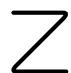
\includegraphics[keepaspectratio]{images/part002_ecaa53ed.jpg}}

\[
\int_ {n \pi} ^ {(n + 1) \pi} \frac {\sin^ {2} t}{t} d t \geqslant \frac {1}{(n + 1) \pi} \int_ {0} ^ {\pi} \sin^ {2} t d t \geqslant \frac {1}{2} \int_ {n + 1} ^ {n + 2} \frac {d t}{t},
\]

由此得

\[
\int_ {\pi} ^ {n \pi} \frac {\sin^ {2} t}{t} d t \geqslant \frac {1}{2} \int_ {2} ^ {n + 1} \frac {d t}{t}
\]

而积分 \(\int_{1}^{+\infty} dt / t\) 为无穷，尽管 \(\int_{\frac{\pi}{2}}^{x} g(t) dt = -\cos x\) 保持有界（参见 V, p.~260, exerc. 4）。

\subsection{比较关系的求导}

\pandocbounded{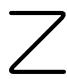
\includegraphics[keepaspectratio]{images/part002_390c97e1.jpg}}

命题 1 (V, p.~228) 与命题 6 (V, p.~230) 没有逆命题：两个函数之间的比较关系 \(\mathbf{f} \preccurlyeq g\) 、 \(\mathbf{f} \ll g\) 、 \(\mathbf{f} \sim \mathbf{c}g\) 的存在（这两个函数在 \(+\infty\) 的一个邻域上可导）并不蕴含它们的导数之间有同样的比较关系，即使对实单调函数 \(f\) 与 \(g\) 亦然。

例如，函数 \(x^{2} + x\sin x + \cos x\) 是单调的且等价于 \(x^{2}\) ，但它的导数 \(x(2 + \cos x)\) 不等价于 \(2x\) 。

另一方面，当先验地假设所考虑函数的导数是可比较的 (V, p.~217) 时，可以导出比较关系。一般地，我们将说定义在区间 \([a, +\infty]\) 上的两个实函数 f 与 g 在 \(+\infty\) 的一个邻域上是 k 阶可比较的，如果在 \(+\infty\) 的一个邻域上，它们各自除在一个可数集的点处外都有规则的 \(k^{th}\) 导数，并且在这个邻域上 \(f^{(k)}\) 与 \(g^{(k)}\) 具有常号（在其有定义的集上）且是可比较的。

我们约定称两个可比较的实函数（V, p.~217）为 0 阶可比较的。

命题 7. 若两个实函数 \(f, g\) 是 1 阶可比较的，则它们是可比较的；此外，关系 \(f \ll g\) （相应地， \(f \sim cg\) ， \(c\) 为常数）蕴含 \(f' \ll g'\) （相应地， \(f' \sim cg'\) ），除非 \(g\) 等价于一个非零常数。

现在，由于 \(f'\) 与 \(g'\) 在一个区间 \([x_0, +\infty[\) 上具有常号， \(f\) 与 \(g\) 都在这个区间上单调，故当 \(x\) 趋于 \(+\infty\) 时趋于一个有限或无穷的极限。显然， \(f\) 与 \(g\) 当 \(x\) 趋于 \(+\infty\) 时是可比较的（若这两个极限之一有限且 \(\neq 0\) ，或者一个为零而另一个为无穷）。若 \(f\) 与 \(g\) 都趋于 0，可以写 \(f(x) = -\int_x^{+\infty} f'(t) dt\) ， \(g(x) = -\int_x^{+\infty} g'(t) dt\) ；由于 \(f'\) 与 \(g'\) 可比较， \(f\) 与 \(g\) 亦然，且 \(f\) 与 \(g\) 之间的比较关系等同于 \(f'\) 与 \(g'\) 之间的比较关系（由 V, p.~20 的命题 6）。类似地，若 \(f\) 与 \(g\) 都有一个无穷极限，则有 \(f(x) = f(x_0) + \int_{x_0}^x f'(t) dt\) ， \(g(x) = g(x_0) + \int_{x_0}^x g'(t) dt\) ；V, p.~230 的命题 6 仍然表明 \(f\) 与 \(g\) 可比较，且 \(f\) 与 \(g\) 之间的比较关系等同于 \(f'\) 与 \(g'\) 之间的比较关系。为完成证明，剩下考虑 \(g\) 趋于 \(\pm \infty\) 而 \(f\) 趋于一个常数的情形；这时不可能有 \(f' \succcurlyeq g'\) ，因为那样由 V, p.~218 的命题 1 将可推出积分 \(\int_{x_0}^{+\infty} g'(t) dt\) 收敛；由于已假设 \(f'\) 与 \(g'\) 可比较，必有 \(f' \ll g'\) 。

推论. 若两个实函数 \(f, g\) 是 \(k \geqslant 1\) 阶可比较的，则它们是 \(p\) 阶可比较的（对 \(0 \leqslant p \leqslant k\) ）；此外，关系 \(f \ll g\) （相应地， \(f \sim cg\) ）蕴含 \(f^{(k)} \ll g^{(k)}\) （相应地， \(f^{(k)} \sim cg^{(k)}\) ），除非诸导数 \(g^{(p)}\) 之一（ \(0 \leqslant p \leqslant k - 1\) ）等价于一个常数 \(\neq 0\) 。

事实上，由于 \(f^{(k)}\) 与 \(g^{(k)}\) 在一个区间 \([x_0, +\infty[\) 上具有常号，由此得出 \(f^{(k-1)}\) 与 \(g^{(k-1)}\) 在这个区间上单调，故在 \(+\infty\) 的一个邻域上具有常号；此外，V, p.~232 的命题 7 表明 \(f^{(k-1)}\) 与 \(g^{(k-1)}\) 可比较，于是推论由递归地应用命题 7 而得。

注. 1) 命题 7 中对 \(g\) 的限制是本质的。例如，有 \(\frac{1}{x} \ll 1 + \frac{1}{x}\) ，尽管两边的导数是等价的；类似地 \(1 + \frac{1}{x} \sim 1 + \frac{1}{x^2}\) ，但 \(1 / x^2 \gg 2 / x^3\) 。

\begin{enumerate}
\def\labelenumi{\arabic{enumi})}
\setcounter{enumi}{1}
\item
  尽管 \(f\) 与 \(g\) 是 \(k\) 阶可比较的，一个函数 \(f_{1}\) （等价于 \(f\) 的）不必是 \(k\) 阶可比较的（与 \(g\) ）；但若假设 \(f_{1}\) 是 \(k\) 阶可比较的（与 \(f\) ），且诸导数 \(f^{(p)}\) （ \(0 \leqslant p \leqslant k - 1\) ）无一等价于一个非零常数，则它将是如此。
\item
  若 f 与 g 是 k 阶可比较的，这对 hf 与 hg 未必成立，即使对像 \(h(x) = x\) 这样简单的单调函数 h 亦然 (V, p.~260, exerc. 3)；同样，1/f 与 1/g 也不必然是 k 阶可比较的 (V, p.~259, exerc. 1)。
\end{enumerate}

\subsection{原函数的主部}

设 \(f\) 是一个规则实函数， \(\neq 0\) 且在一个区间 \([a, +\infty[\) 上具有常号；下面的命题使我们在某些情形能够得到原函数 \(\int_{x}^{+\infty} f(t) dt\) 的主部（若 \(\int_{a}^{+\infty} f(t) dt\) 收敛），以及原函数 \(\int_{a}^{x} f(t) dt\) 的主部（若 \(\int_{a}^{+\infty} f(t) dt\) 为无穷）：

命题 8. 置 \(\mathrm{F}(x) = \int_{x}^{+\infty} f(t) dt\) （若 \(\int_{a}^{+\infty} f(t) dt\) 收敛），而置 \(\mathrm{F}(x) = \int_{a}^{x} f(t) dt\) （若 \(\int_{a}^{+\infty} f(t) dt\) 为无穷）。设 \(\log |f|\) 与 \(\log x\) 是 1 阶可比较的。

\(1^{\circ}\) 若 \(f\) 是有限阶 \(\mu \neq -1\) 的（相对于 \(x\) ），则有

\[
\mathrm{F} (x) \sim \frac {1}{| \mu + 1 |} x f (x).\tag{1}
\]

\(2^{\circ}\) 若 \(f\) 相对于 \(x\) 是无穷阶的，且 \(f / f'\) 与 \(x\) 是 1 阶可比较的，则有

\[
\mathrm{F} (x) \sim \frac {(f (x)) ^ {2}}{| f ^ {\prime} (x) |}.\tag{2}
\]

应当注意，假设蕴含 \(f(x)\) 相对于 \(x\) 有确定的阶 (V, p.~219)。

\(1^{\circ}\) 若 \(f\) 是 \(\mu \neq 0\) 阶的（相对于 \(x\) ），则有 \(\log |f| \sim \mu \log x\) ，于是，由于 \(\log |f|\) 与 \(\log x\) 是 1 阶可比较的，由 V, p.~232 的命题 7 有 \(f'/f \sim\) \(\mu/x\) ，由此 \(xf' \sim \mu f\) 。若 \(\mu > -1\) ，则有 \(f(x) \gg x^{\mu-\varepsilon}\) （对每个 \(\varepsilon > 0\) ），从而 (V, p.~229, prop. 2) 积分 \(\int_{a}^{+\infty} f(t) dt\) 为无穷。可以写 \(F(x) = \int_{a}^{x} f(t) dt = xf(x) - af(a) - \int_{a}^{x} tf'(t) dt\) ，由此再次得到

\[
\int_ {a} ^ {x} \left(f (t) + t f ^ {\prime} (t)\right) d t = x f (x) - a f (a);
\]

由于 \(\mu \neq -1\) ，有 \(f(x) + xf'(x) \sim (\mu + 1)f(x)\) ，故 (V, p.~230, prop. 6)

\[
\int_ {a} ^ {x} \left(f (t) + t f ^ {\prime} (t)\right) d t \sim (\mu + 1) \mathrm{F} (x),
\]

这就在这种情形证明了 (1)。若 \(\mu = 0\) ，同样有 \(xf'(x) \ll f(x)\) ，它再次给出 \(f(x) + xf'(x) \sim f(x)\) 。当 \(\mu < -1\) 时论证类似（在 \(\int_{a}^{+\infty} f(t) dt\) 收敛的情形）。

\(2^{\circ}\) 若 \(f\) 是 \(+\infty\) 阶的（相对于 \(x\) ），则有 \(\log |f| \gg \log x\) ，故 (V, p.~232, prop. 7) \(f'/f \gg 1/x\) ，或者再令 \(g(x) = f(x)/f'(x)\) ，有 \(g(x) \ll x\) ；此外，由于 \(f(x) \gg x^{\alpha}\) （对每个 \(\alpha > 0\) ），积分 \(\int_{a}^{+\infty} f(t) dt\) 为无穷。可以写

\[
\mathrm{F} (x) = \int_ {a} ^ {x} f (t) d t = \int_ {a} ^ {x} g (t) f ^ {\prime} (t) d t = g (x) f (x) - g (a) f (a) - \int_ {a} ^ {x} f (t) g ^ {\prime} (t) d t;
\]

由于 \(g\) 与 \(x\) 是 1 阶可比较的，从关系 \(g(x) \ll x\) 可推出 (V, p.~232, prop. 7) \(g'(x) \ll 1\) ，从而 \(fg' \ll f\) ，于是 (V, p.~230, prop.6)

\[
\int_ {a} ^ {x} f (t) g ^ {\prime} (t) d t \ll \mathrm{F} (x),
\]

这就建立了关系式 (2)。当 \(f\) 是 \(-\infty\) 阶的（相对于 \(x\) ）时证明类似（在 \(\int_{a}^{+\infty} f(t) dt\) 收敛的情形）。

设 E 是一个比较尺度（对趋于 \(+\infty\) 的实 x 而言），由在 \(+\infty\) 的一个邻域上具有常号的非零实函数组成，使得 \(x \in E\) ，且 E 中两个函数的乘积与商仍属于 E (V, p.~221 and p.~224)。若一个在 \(+\infty\) 的一个邻域上具有常号的规则函数 f 相对于 E 有主部 cg，则 \(\int_{x}^{+\infty} f(t) dt\) （相应地， \(\int_{a}^{x} f(t) dt\) ，视情形而定）将等价于 \(c \int_{x}^{+\infty} g(t) dt\) （相应地， \(c \int_{a}^{x} g(t) dt\) ）；若函数 g 满足 V, p.~233 的命题 8 的假设，且（当 V, p.~233 的公式 (2) 适用时）知道 \(g'\) 相对于 E 的一个主部，则由此将有 \(\int_{x}^{+\infty} f(t) dt\) （相应地， \(\int_{a}^{x} f(t) dt\) ）相对于 E 的一个主部。

例. 1) 函数 \(1 / \log x\) 相对于 \(x\) 是 0 阶的且满足 V, p.~233 的命题 8 的条件；于是

\[
\int_ {a} ^ {x} \frac {d t}{\log t} \sim \frac {x}{\log x}.
\]

\begin{enumerate}
\def\labelenumi{\arabic{enumi})}
\setcounter{enumi}{1}
\tightlist
\item
  函数 \(e^{x^2}\) 是 \(+\infty\) 阶的（相对于 \(x\) ）且满足命题 8 的条件，故
\end{enumerate}

\[
\int_ {a} ^ {x} e ^ {t ^ {2}} d t \sim \frac {1}{2 x} e ^ {x ^ {2}}.
\]

在附录 (V, p.~252) 中我们将定义一类函数，对它们命题 7 与命题 8 总是适用的。

注. 命题 8 不直接应用于一个函数 \(f\) （ \(-1\) 阶的，相对于 \(x\) ）。但这时可以写 \(f(x) = f_1(x) / x\) ，其中 \(f_1\) 相对于 \(x\) 是 0 阶的。例如设 \(\int_{a}^{+\infty} f(t) dt\) 为无穷；则

\[
\mathrm{F} (x) = \int_ {a} ^ {x} f (t) d t = \int_ {a} ^ {x} \frac {1}{t} f _ {1} (t) d t = \int_ {\log a} ^ {\log x} f _ {1} \left(e ^ {u}\right) d u.
\]

若函数 \(f_{1}(e^{y})\) 满足命题 8 的假设且有一个 \(\neq -1\) 的阶（相对于 \(y\) ）（也就是说，若 \(f_{1}(x)\) 有一个 \(\neq -1\) 的阶（相对于 \(\log x\) ）），则公式 (1) 与 (2) 仍能使我们得到 \(F(x)\) 的一个主部。例如，设 \(f(x) = \frac{\exp(\sqrt{\log x})}{x\log x}\) ；由于 \(\exp(\sqrt{\log x})\) 相对于 \(x\) 是 0 阶的， \(f\) 是 \(-1\) 阶的；这里有 \(f_{1}(e^{y}) = e^{\sqrt{y}} / y\) ，且这个函数是 \(+\infty\) 阶的（相对于 \(y\) ）；命题 8 适用并给出 \(\int_{\alpha}^{y} e^{\sqrt{u}} / u du \sim 2e^{\sqrt{y}} / \sqrt{y}\) ；回到变量 \(x\) ，我们有 \(\int_{a}^{x} \frac{\exp(\sqrt{\log t})}{t\log t} dt \sim \frac{2\exp(\sqrt{\log x})}{\sqrt{\log x}}\) 。

\subsection{原函数的渐近展开}

设 E 是 \(+\infty\) 的一个邻域上的一个比较尺度，由 \(\neq 0\) 的、在 \(+\infty\) 的一个邻域上具有常号的实函数组成；设 f 是定义在一个区间 \([a, +\infty[\) 上的规则向量函数，取值于一个完备赋范空间 E 中，容许一个渐近展开

\[
\mathbf {f} = \sum_ {\lambda \leqslant \alpha} \mathbf {a} _ {\lambda} g _ {\lambda} + \mathbf {r} _ {\alpha}
\]

（精确到 \(g_{\alpha}\) ，相对于 E）。进一步假设每个原函数 \(\int_{a}^{x} g(t) dt\) （函数 \(g \in E\) 的）相对于 E 容许一个渐近展开。在这些情形下我们将看到，可以得到 \(\mathbf{F}(x) = \int_{a}^{x} \mathbf{f}(t) dt\) 相对于 E 的一个渐近展开。我们区分两种情形：

\(1^{\circ}\int_{a}^{+\infty}g_{\alpha}(t)dt\) 为无穷；则有 \(\int_{a}^{x}\mathbf{r}_{\alpha}(t)dt\ll \int_{a}^{x}g_{\alpha}(t)dt\) (V,p.230, prop. 6)；由假设可以得到 \(\sum_{\lambda \leqslant \alpha}\mathbf{a}_{\lambda}\int_{a}^{x}g_{\lambda}(t)dt\) 的一个渐近展开

（精确到某个 \(g_{\rho}\) ）(V, p.~222)；若 \(cg_{\sigma}\) 是 \(\int_{a}^{x} g_{\alpha}(t) dt\) 的主部，则由此将有 \(\int_{a}^{x} \mathbf{f}(t) dt\) 的一个精确到 \(g_{\min(\rho, \sigma)}\) 的渐近展开，其所有项的范数不定递增。

\(2^{\circ}\int_{a}^{+\infty}g_{\alpha}(t)dt\) 收敛；设 \(\beta\) 是指标 \(\lambda \leqslant \alpha\) 中最小的使 \(\mathbf{a}_{\lambda}\neq 0\) 且使 \(\int_{a}^{+\infty}g_{\lambda}(t)dt\) 收敛者；积分

\[
\mathbf {C} = \int_ {a} ^ {+ \infty} \left(\mathbf {f} (t) - \sum_ {\lambda <   \beta} \mathbf {a} _ {\lambda} g _ {\lambda} (t)\right) d t
\]

这时收敛，且可以写

\[
\mathbf {F} (x) = \sum_ {\lambda <   \beta} \mathbf {a} _ {\lambda} \int_ {a} ^ {x} g _ {\lambda} (t) d t + \mathbf {C} - \sum_ {\beta \leqslant \lambda \leqslant \alpha} \mathbf {a} _ {\lambda} \int_ {x} ^ {+ \infty} g _ {\lambda} (t) d t - \int_ {x} ^ {+ \infty} \mathbf {r} _ {\alpha} (t) d t.
\]

则 \(\int_{x}^{+\infty}\mathbf{r}_{\alpha}(t)dt\ll \int_{x}^{+\infty}g_{\alpha}(t)dt\) ；若 \(cg_{\sigma}\) 是 \(\int_{x}^{+\infty}g_{\alpha}(t)dt\) 的主部，且若有

\[
\sum_ {\lambda <   \beta} \mathbf {a} _ {\lambda} \int_ {a} ^ {x} g _ {\lambda} (t) d t + \mathbf {C} - \sum_ {\beta \leqslant \lambda \leqslant \alpha} \mathbf {a} _ {\lambda} \int_ {x} ^ {+ \infty} g _ {\lambda} (t) d t
\]

的一个渐近展开（精确到 \(g_{\rho}\) ），则由此将有 \(\mathbf{F}\) 的一个精确到 \(g_{\min(\rho, \sigma)}\) 的渐近展开。

于是问题归结为求 E 中函数的原函数相对于 E 的渐近展开。我们已经看到，在某些关于 E 的假设下，V, p.~233 的命题 8 如何给出这种原函数的主部。此外，命题 8 的证明给出 V, p.~233 的公式 (1) （相应地， (2)）两边之差的表达式，其形式为函数 \(\frac{1}{|\mu+1|}\left(xf'(x)+f(x)\right)-f(x)\) （相应地， \(f(x)g'(x)\) ，其中 \(g=f/f'\) ）的一个原函数；在构成这个新原函数的主部（作为 (1) （相应地， (2)）右边的一个渐近展开）时，就得到所求展开的右边（参见 V, p.~247-255）。

例. 1) 设 \(f(x) = 1 / \log x\) （ \(x > 1\) ）；我们已经看到 \(\int_{a}^{x} dt / \log t \sim x / \log x\) ，且差 \(\int_{a}^{x} \frac{dt}{\log t} - \frac{x}{\log x}\) 是 \(1 / (\log x)^2\) 的一个原函数；对这个函数可再次应用命题 8，从而得到 \(\int_{a}^{x} dt / (\log t)^2 \sim x / (\log x)^2\) 。由递归于是得到展开

\[
\begin{array}{l} \int_ {a} ^ {x} \frac {d t}{\log t} = \frac {x}{\log x} + \frac {x}{(\log x) ^ {2}} \\ \qquad + \frac {2 x}{(\log x) ^ {3}} + \dots + (n - 1)! \frac {x}{(\log x) ^ {n}} + o \left(\frac {x}{(\log x) ^ {n}}\right). \end{array}
\]

注意，不论 n 为何，这个展开的所有项都随 x 趋于 \(+\infty\) 。

\begin{enumerate}
\def\labelenumi{\arabic{enumi})}
\setcounter{enumi}{1}
\tightlist
\item
  设 \(f(x) = \frac{e^x}{x^2 + 1}\) ；可以写 \(f(x) = \frac{e^x}{x^2} - \frac{e^x}{x^4} + o_1\left(\frac{e^x}{x^4}\right)\) 。命题 8 给出展开
\end{enumerate}

\[
\int_ {a} ^ {x} \frac {e ^ {t}}{t ^ {2}} d t = \frac {e ^ {x}}{x ^ {2}} + \frac {2 e ^ {x}}{x ^ {3}} + \frac {6 e ^ {x}}{x ^ {4}} + o _ {2} \left(\frac {e ^ {x}}{x ^ {4}}\right), \quad \int_ {a} ^ {x} \frac {e ^ {t}}{t ^ {4}} d t = \frac {e ^ {x}}{x ^ {4}} + o _ {3} \left(\frac {e ^ {x}}{x ^ {4}}\right)
\]

由此，把两式相加，

\[
\int_ {a} ^ {x} \frac {e ^ {t}}{t ^ {2} + 1} d t = \frac {e ^ {x}}{x ^ {2}} + 2 \frac {e ^ {x}}{x ^ {3}} + 5 \frac {e ^ {x}}{x ^ {4}} + o _ {4} \left(\frac {e ^ {x}}{x ^ {4}}\right).
\]

\section{应用于正项级数}
